\documentclass[10pt,journal,compsoc]{IEEEtran}

\ifCLASSOPTIONcompsoc
  % IEEE Computer Society needs nocompress option
  % requires cite.sty v4.0 or later (November 2003)
  \usepackage[nocompress]{cite}
\else
  % normal IEEE
  \usepackage{cite}
\fi

\usepackage{graphicx}
\usepackage{tikz}
\usepackage{amsmath}
\usepackage{listings}
\usepackage{multicol,lipsum}
\lstset{
    %%numbers=left,
    breaklines=true,
    tabsize=2,
    basicstyle=\ttfamily,
    language = c++,
}

\ifCLASSINFOpdf

\else

\fi

\hyphenation{op-tical net-works semi-conduc-tor}


\begin{document}

\hyphenpenalty=100000

\title{Microbot - Rescuebot}


\author{Miguel~Rodriguez Delgado, Marwa Mohammed Nabwey Hassan, Asadujaman Nur, Vincent Chinedu Obigwe, Abeeb Opeyemi Nureni and Charles Arsenal Okere * ~Hochschule Hamm-Lippstadt}

\IEEEtitleabstractindextext{%
\begin{abstract}
Over the last decade, the technology of  Smart Home has been rapidly improved to serve increasing safety and reliability in modern houses.This paper aims to describe the design of our smart home system that we build, we did include a wide range of aspects as  Home security, Lightning system, controlling home Windows and Home Heating, ventilation, and air conditioning (HVAC). All the above is executed with the help of  an Arduino microcontroller and sensors, a smart home security system DS2 is used to notify the user if there are any guests by the door and alert the home users by sending a short message when suspicious activity occurs, as well as controlling turning on/off home light and window and other appliances like heater and AC, which could be easy, rather than using the traditional method of the home switch, we ended up implementing a user-friendly, reliable and compact based smart home system. [Marwa Hassan] 
\end{abstract}

\begin{IEEEkeywords}
Rescue robot, Puzzle solving, Path finder, System Modelling, UML, SysML, Prototyping, SolidWorks, System requirements, Rescue robot, Spider-bot, Robot Spider, Lifesaver, Coding, simulation, maps, programming .
\end{IEEEkeywords}}


\maketitle


\IEEEdisplaynontitleabstractindextext

\IEEEpeerreviewmaketitle



\section{Introduction (Vincent  Obigwe)}\label{sec:introduction}

\IEEEPARstart{A} robot may not injure a human being or through inaction, allow a human being to come to harm - Isaac Asimov. This is the true case of our rescue robot that hopes to rescue accident and emergency victims. The project is divided into three distinct but inseparable parts; the system engineering, the prototyping and the programming.

The system engineering served as a watering ground where it all started. From developing the requirement diagram to the use case diagram, it has all been about making the robot better and smarter, and also gaining a first class understanding of what the various tasks are. The system engineering provided a clear understanding and implementation pathway for the robot.

After understanding the system requirements and having a mental map of how to go about the robot development, Prototyping comes into effect. With prototyping we were able to design the robot first with a sketch drawing, and later with the help of a CAD software SolidWorks. The designs are done in accordance with the specifications and standards. The last part of prototyping is identifying the various electrical/electronics parts to be used in the development of the robot and confirming that it fits. 

A robot is made as smart as it is with the help of the software. This is where the programming aspect of the project comes in. We were able to write codes that detect the movement of robots. Though the codes written does not have a direct impact on our robot, we made use of a robot stimulation to write codes that were appreciated to take the best route, and also save energy. 

The overall glory of the project is shared by the tripartite contribution of the system engineering, prototyping and software programming. It is also believed that a lot of modifications and extensions can be added to our robot.

\section{System Modelling}

\subsection{Context Diagram (Vincent  Obigwe)}

Every system is context based. By context we meant a situation in which something exists or happens, that can help explain it. Context diagrams helps us to better understand our system and how they communicate and interact with our environment. Some of the main examples of a context diagram includes but not limited to the following:

a. Parametric Constraint Diagram 

b. System Breakdown bdd

c. SysMLContext Structure 


\subsubsection{Parametric constraint Diagram}

\begin{figure}[!h]
\includegraphics[scale=0.26]{parametric}
\caption{Parametric constraint Diagram}
\label{fig:parametricDiagram}
\end{figure}

Parametric Diagrams are regarded as a specialized block diagram that helps the system modeler to combine the system behaviour and system structure models with an engineering analysis models example, performance, reliability and mass property model. This helps in determining the various constraints the systems could face.

From our parametric constraint diagram, we outlined using various blocks the various constraints in our system. These includes but not limited to Communication, Terrain, Power source, Weight limit etc. All the identified constraints has accompanying values that helps to properly detail it for better understanding and completeness. Fig \ref{fig:parametricDiagram}

\subsubsection{System Breakdown}

This is a diagram showing the systems, environment’s and the various user components. It further shows the interrelationships between the various componentsand their relationships. 

In our rescue robot system breakdown, it can  be observed that the relationships, dependency relation some casses multiplicities was highlighted making it very detailed. The Rescue Robot System includes the body, the communication system, the Audio and Video system, the Motors, positioning system, power system sensors and controller. The controller software is directly dependent on the controller which happens to also have a composition relationship with the Rescue Robot system. 

All these individual blocks needs to be present and active for the Resuce Robot to perform optimally. Fig \ref{fig:breakdown}

\begin{figure}[h]
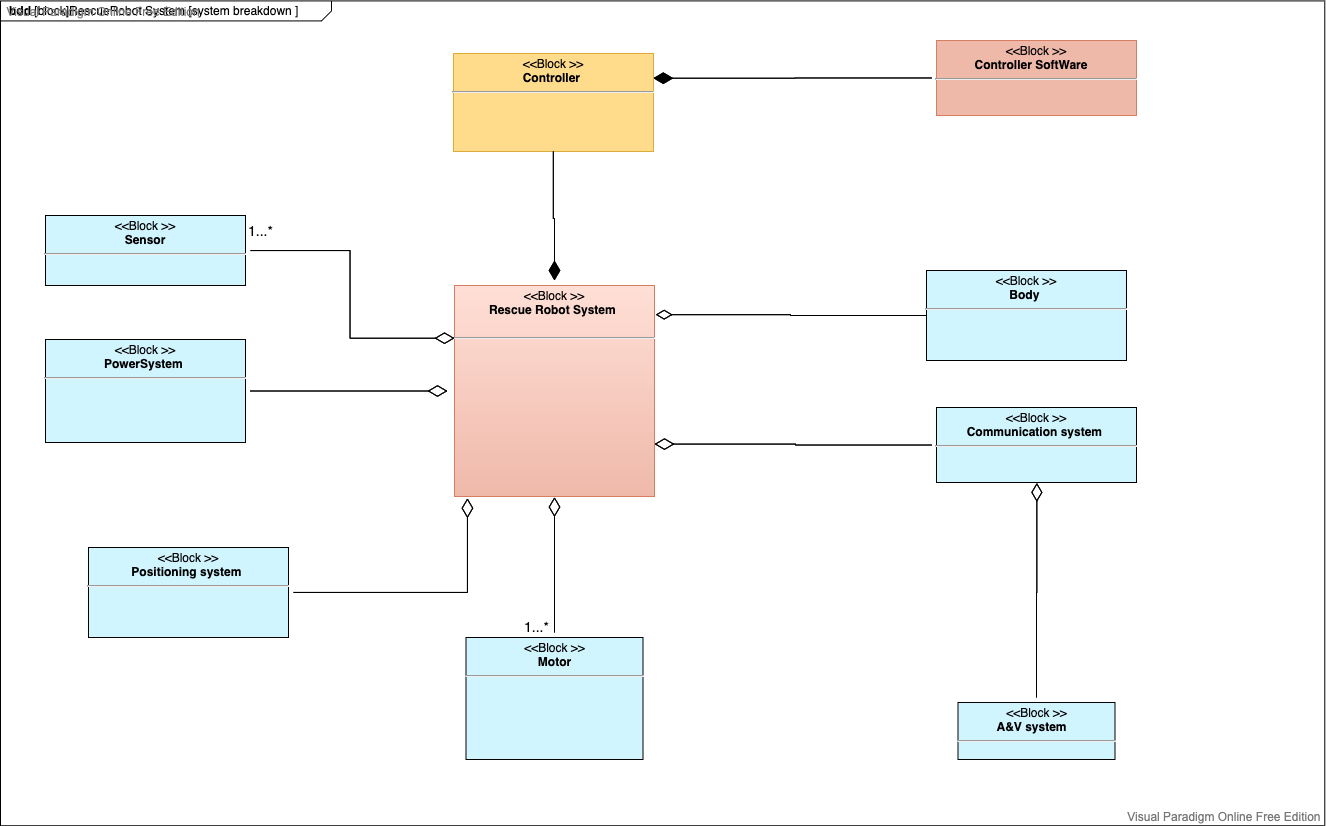
\includegraphics[scale=0.19]{SystemBreakdown}
\caption{System Breakdown}
\label{fig:breakdown}
\end{figure}

\subsubsection{SysML Context Structure }

This is a diagram that represents all external entities that interact with the system. It can be said to be a high level view of a system. 

In the System Context Diagram of our Rescue Robot, it can be seen that we highlighted all the actors, environment and variables.

The actors include the operators. Rescue teams, and victims which act as the stakeholders in the application. Also the main system is identified, together with the external component which is load. The load varies between an object to be rescued or a victim. The external environmental variables were also captured such as the weather, obstacles, water etc.

With all this, it can be seen that the whole system was properly and well studied to be able to extract the full context. Fig \ref{fig:structure}

\begin{figure}[h]
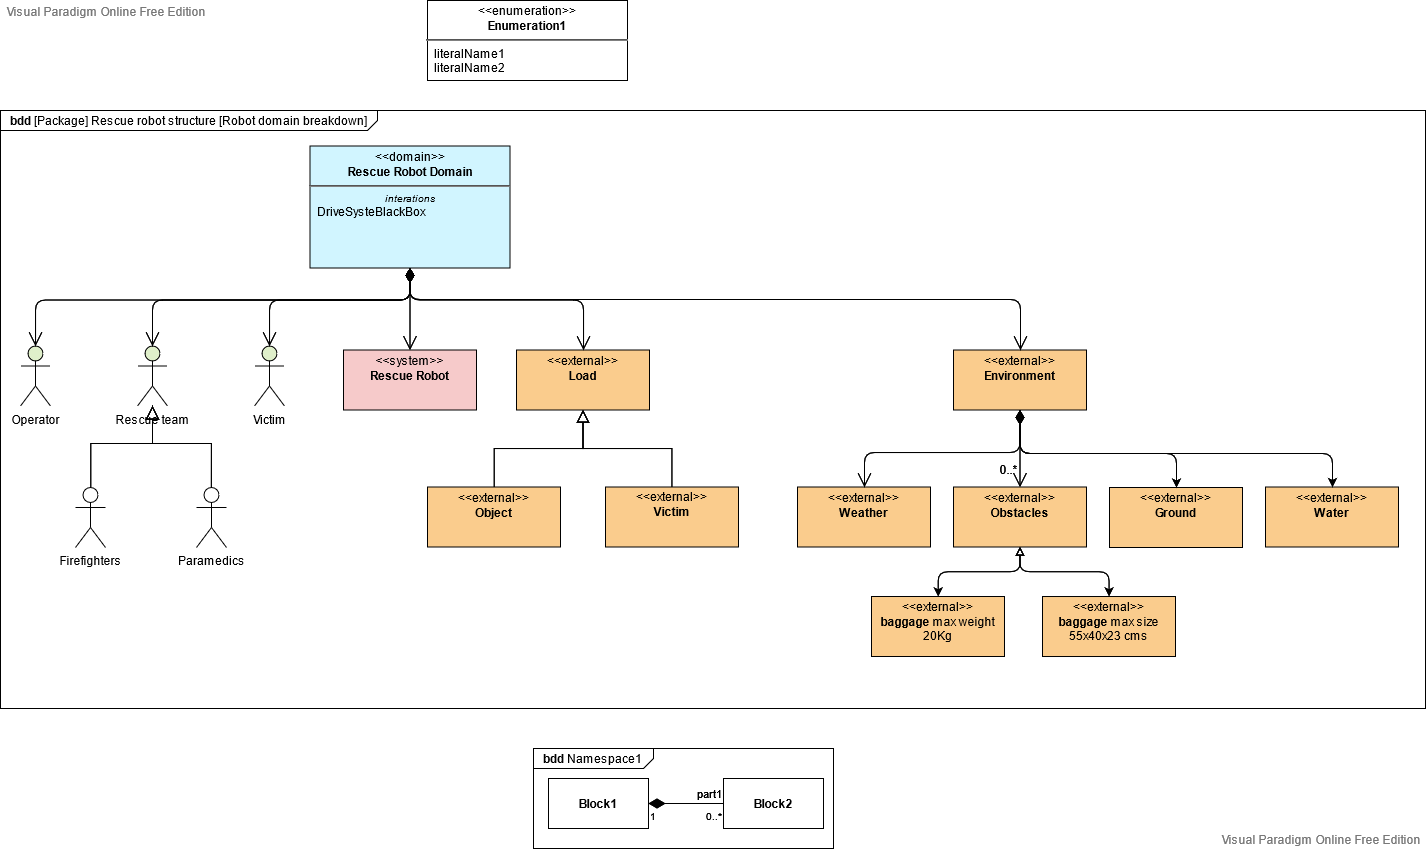
\includegraphics[scale=0.18]{ContextStructure}
\caption{SysML Context Structure}
\label{fig:structure}
\end{figure}

\subsection{Requirement Diagram (Charles Okere)}

Requirement diagram is a static structure diagram that shows the relationships among Requirement (requirement) constructs, model elements that Satisfy (satisfy Dependency) them, and Test Cases that Verify (verify Dependency) them. The purpose of Requirement diagrams is to specify both Functional and Non-Functional Requirements within the model so that they can be traced to other model elements that Satisfy them and Test Cases that Verify them.

As seen in the requirement below, we can see how the functional and non-functional requirements within the model satisfy each other from the  communication aspect to the movement medium down to the measurement of vitals up till when the rescue robot detects objects. Fig \ref{fig:requirements}


\begin{figure}[h]
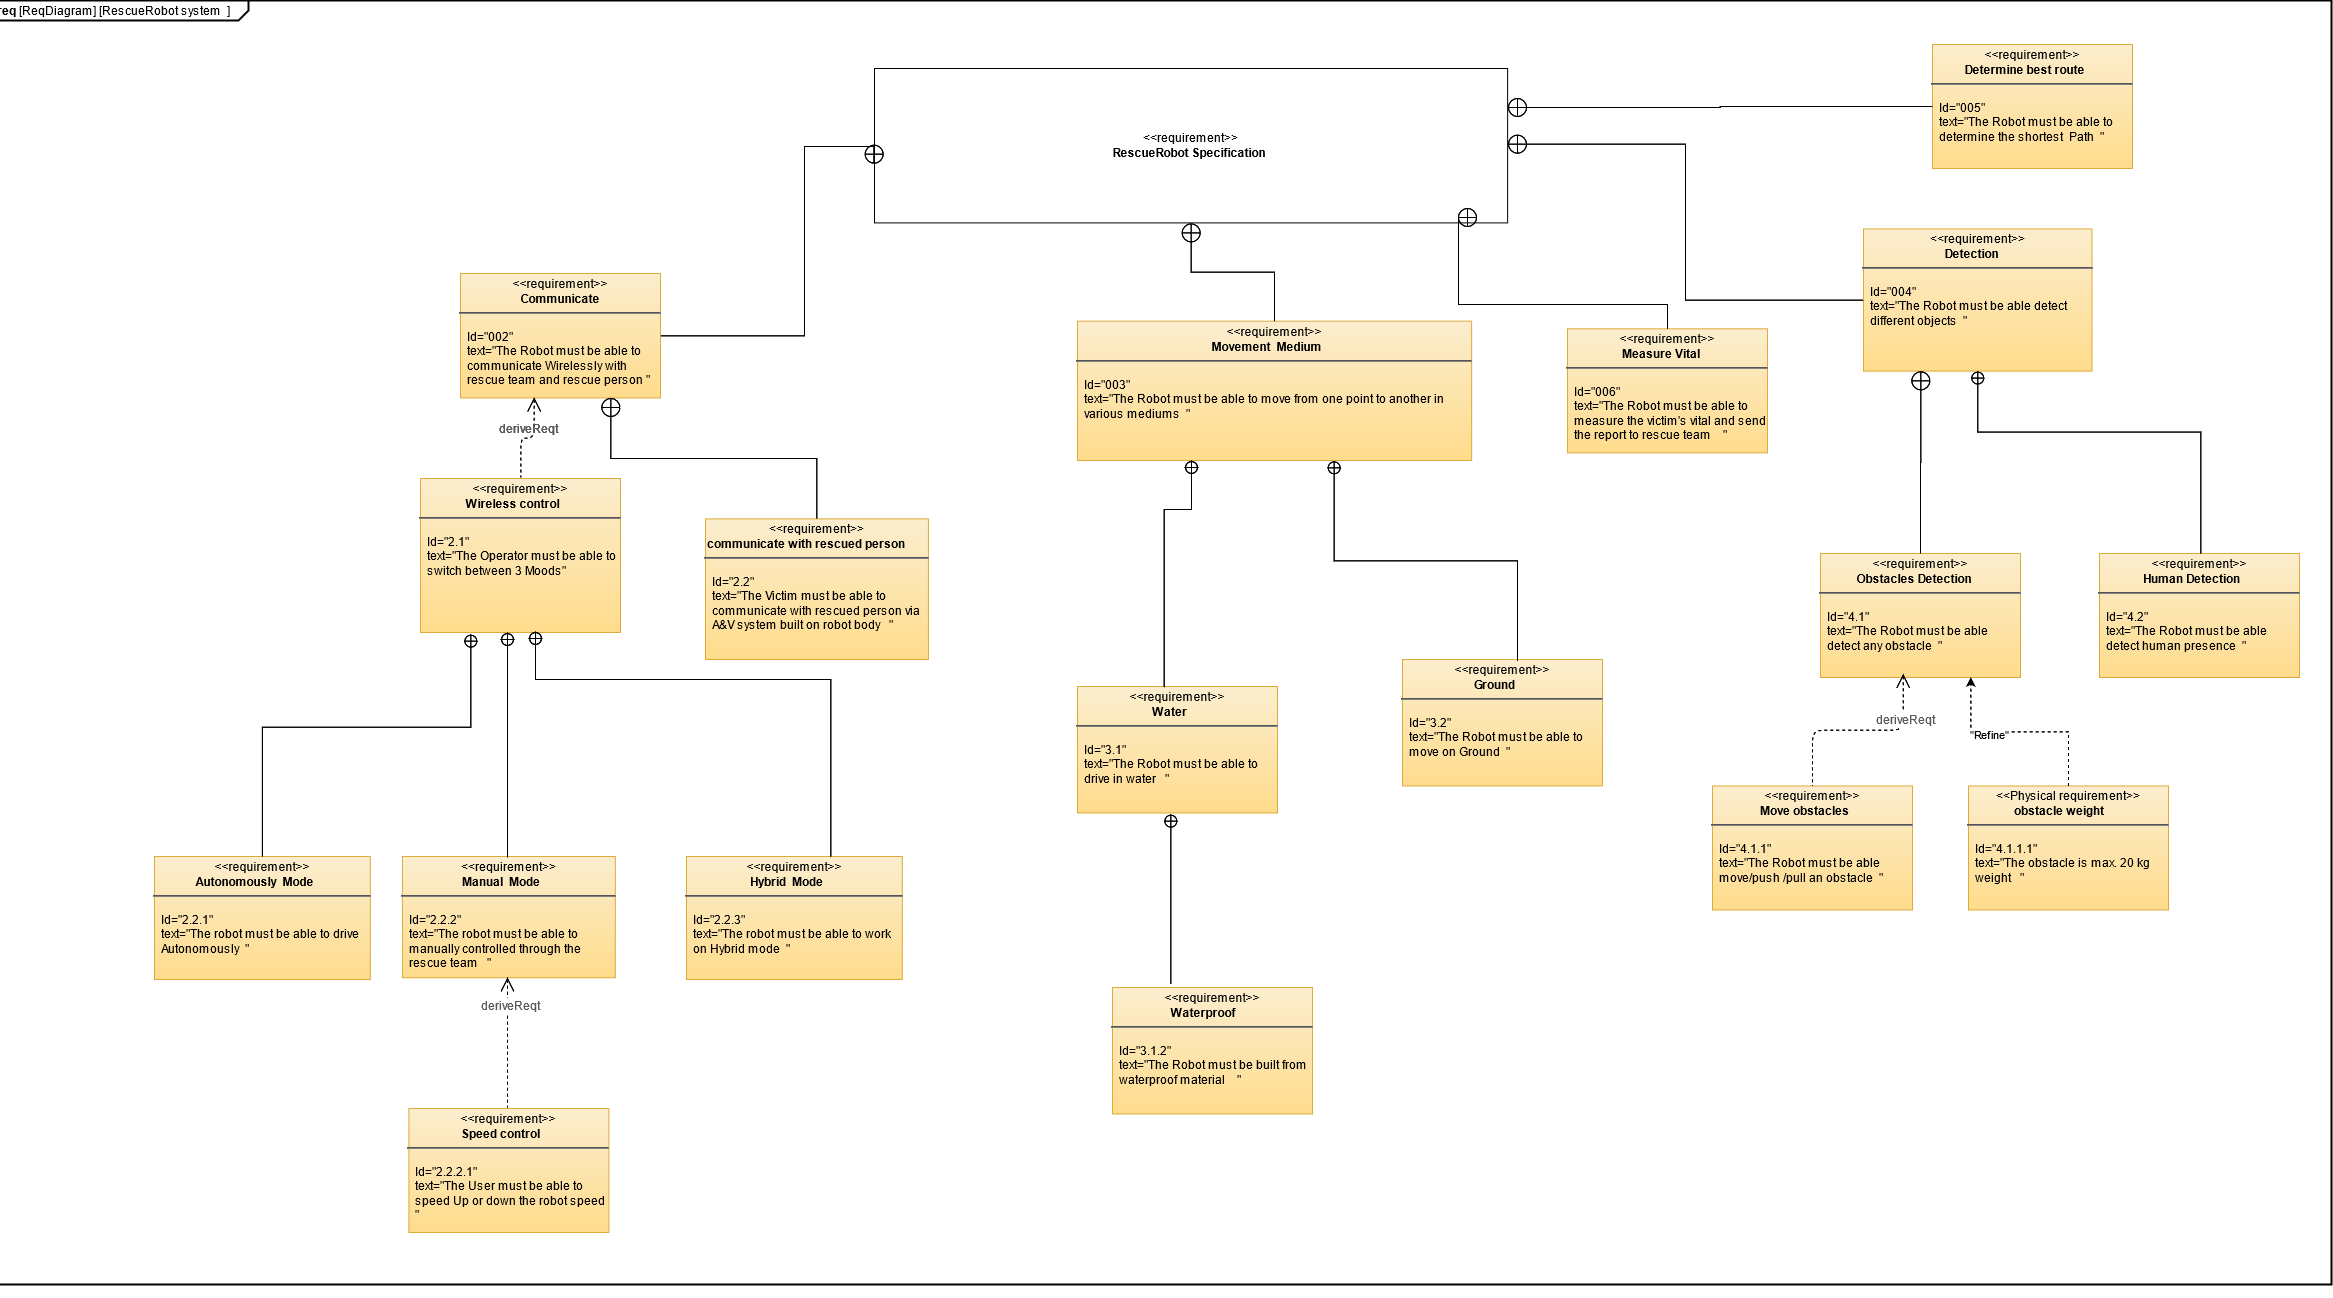
\includegraphics[scale=0.145]{Requirements}
\caption{Requirement Diagram}
\label{fig:requirements}
\end{figure}


\subsection{System Structure (Vincent  Obigwe)}

The system structure diagrams are a set of diagrams that identify the various packs of the system. They include the navigation system, power sub system etc. The various system components would be briefly explained. 

\subsubsection{Navigation System}

The navigation system is the system in charge of providing the robot with directions for autonomous movements.

It includes modules such as the positioning system which serves as the major tool for providing direction with examples such as GPS. The video system Works with the scanner and the autonomous system. All the various components work together with the autonomous system at the center. Fig \ref{fig:navigation}

\begin{figure}[h]
\includegraphics[scale=0.25]{navigation}
\caption{Navigation System}
\label{fig:navigation}
\end{figure}

\subsubsection{Power Sub System}

The power is one of the main driver of the robot. Without power, the robot cannot function at all. 

The power subsystem consists of the battery pack, the switching circuit, voltage regulator, micro-controller, switching circuit output, fused output, stop relay and stop button all interconnected together with various relationships. The human have an external interaction with the system through the stop button, therefore was captured as part of the power sub system. Fig \ref{fig:powerss}

\begin{figure}[h]
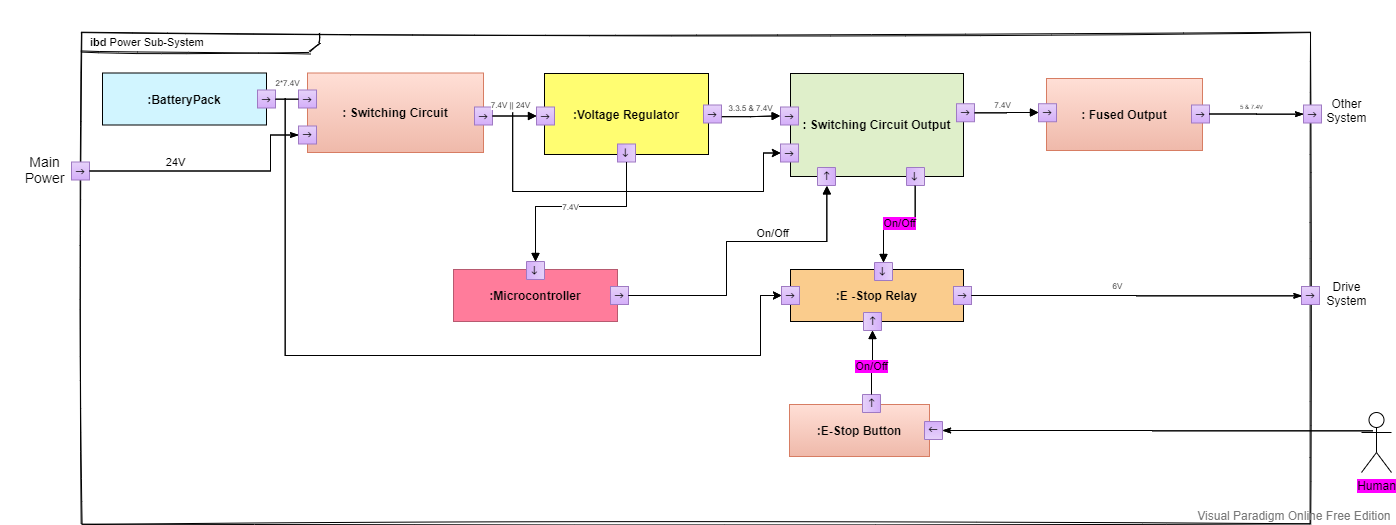
\includegraphics[scale=0.24]{Powerss}
\caption{Power Sub System}
\label{fig:powerss}
\end{figure}

\subsubsection{Robot Drive System}

The drive system is considered to be one of the engine rooms of the robot. This is because it enables locomotion from one point to another. 

In our scenario, the robot drive system enables drive either on the water or land. Our robot drive system is composed of the speed controller, position controller, encoder, motors, drive subsystem for land, and drive subsystem for water all interconnected according to their relationship. This system have a direct connection with the power system. Fig \ref{fig:Drivess}

\begin{figure}[h]
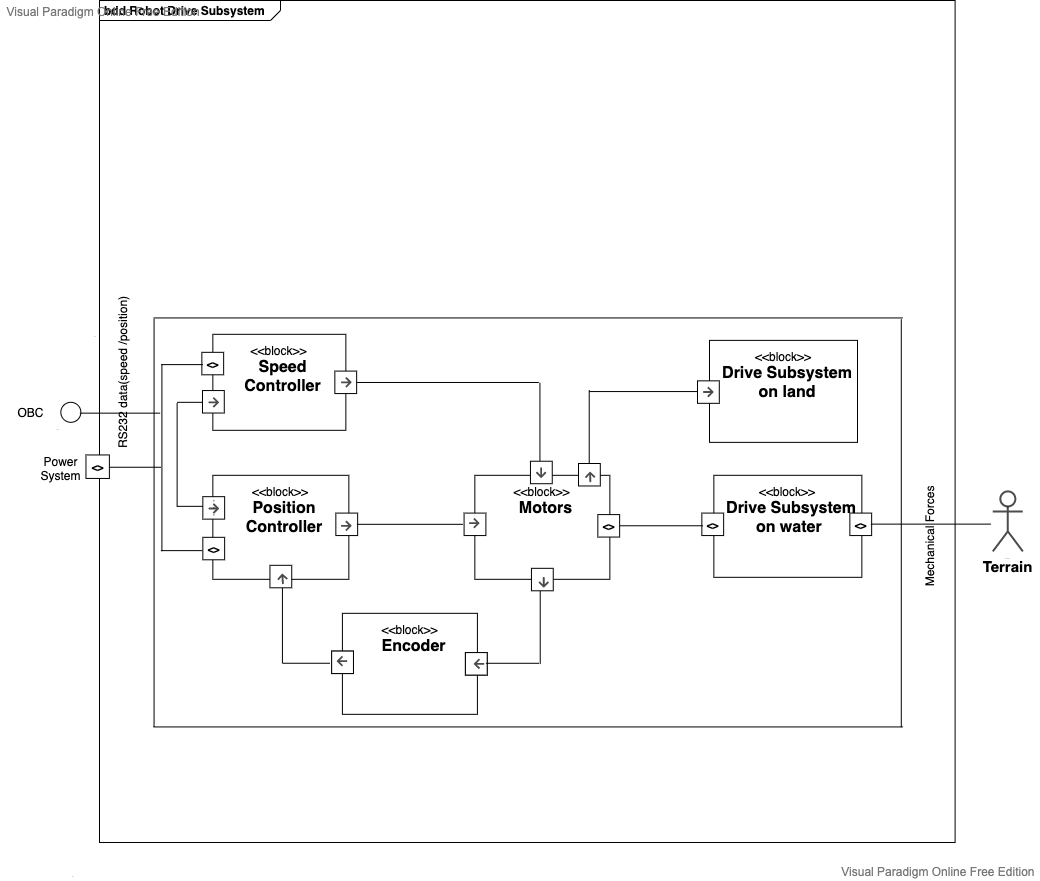
\includegraphics[scale=0.25]{Drivess}
\caption{Robot Drive System}
\label{fig:Drivess}
\end{figure}

\subsubsection{Communication system}

Communication is at the core of every system. The system should have the ability to communicate not just with itself but with the external elements that form part of the system. 

Our Rescue Robot is enabled with a wireless communication system, audio and Video receiver, audio and video sender all connected to the communication unit. The audio and video is received by the robot operator while it is sent by the victim or object through the system. Fig \ref{fig:communicationss}

\begin{figure}[h]
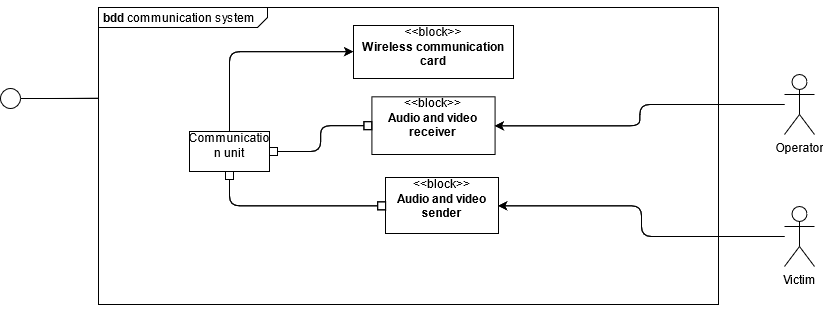
\includegraphics[scale=0.42]{communicationss}
\caption{Communication system}
\label{fig:communicationss}
\end{figure}

\subsubsection{Detection system}

The smartness of any device further comes from its ability to detect the environment and other purposes with which it was built. The detection is usually done with the aid of sensors which now relay the data to the systems for actions. This is why all embedded systems are rigged with various types of sensors that enables it get sensitive information about the environment and also fulfil its special purposes. 

The detection system of our robot measures the vitals of a victim and also detects the environments during movement to either destroy or avoid obstacles. The victim consumes the vital measurement technique of the system while the terrain (land or water) is the subject of the environmental measurement. Fig \ref{fig:detectionss}

\begin{figure}[h]
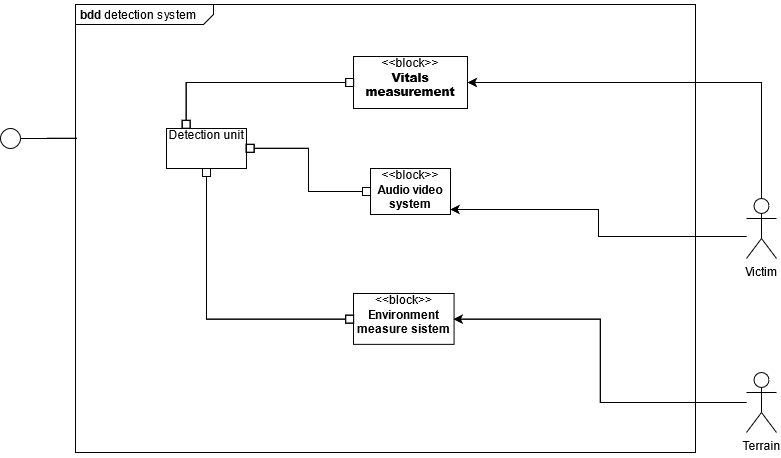
\includegraphics[scale=0.42]{detectionss}
\caption{Detection system}
\label{fig:detectionss}
\end{figure}

\subsubsection{RescueBot system}

This serves as a central hub for combining all the various systems for effective performance and load balancing.

As can be seen from the image, all the systems have a relationship and direct connection with the power systems. Multiplicity is also included in all of them for better clarity and understanding. Fig \ref{fig:RescueBotsys}

\begin{figure}[h]
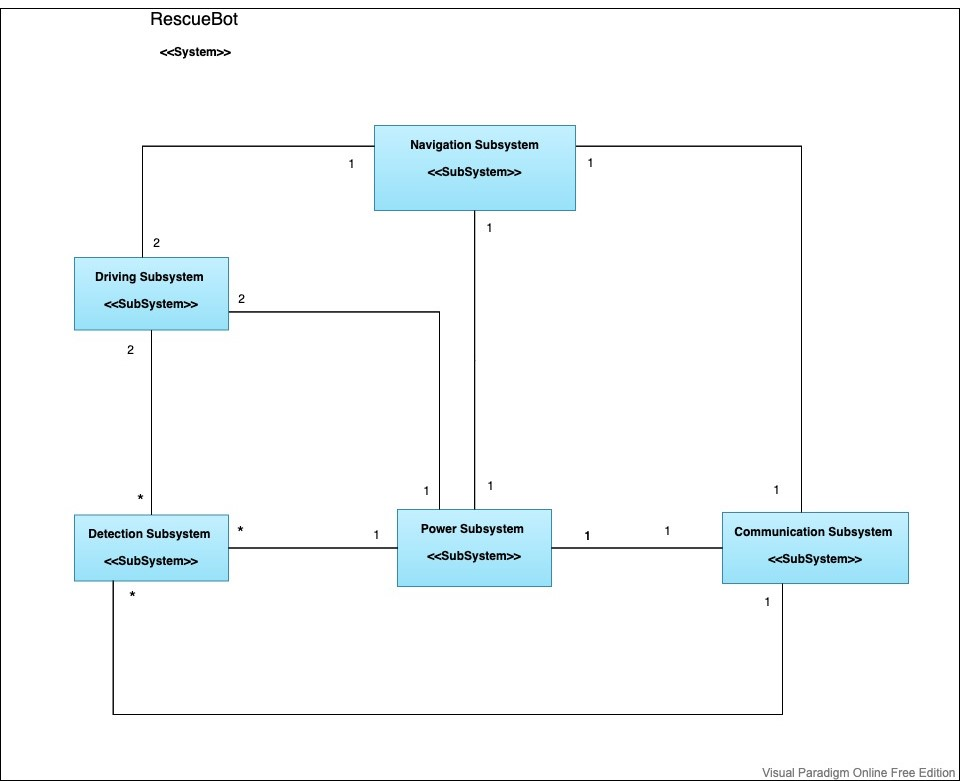
\includegraphics[scale=0.35]{RescueBotsys}
\caption{RescueBot system}
\label{fig:RescueBotsys}
\end{figure}


\subsection{Use Case specification (Charles Okere)}

\subsubsection{Activity Diagram}

Control flows and object flows connect sequential and concurrent activities in an activity diagram.

\begin{figure}[h]
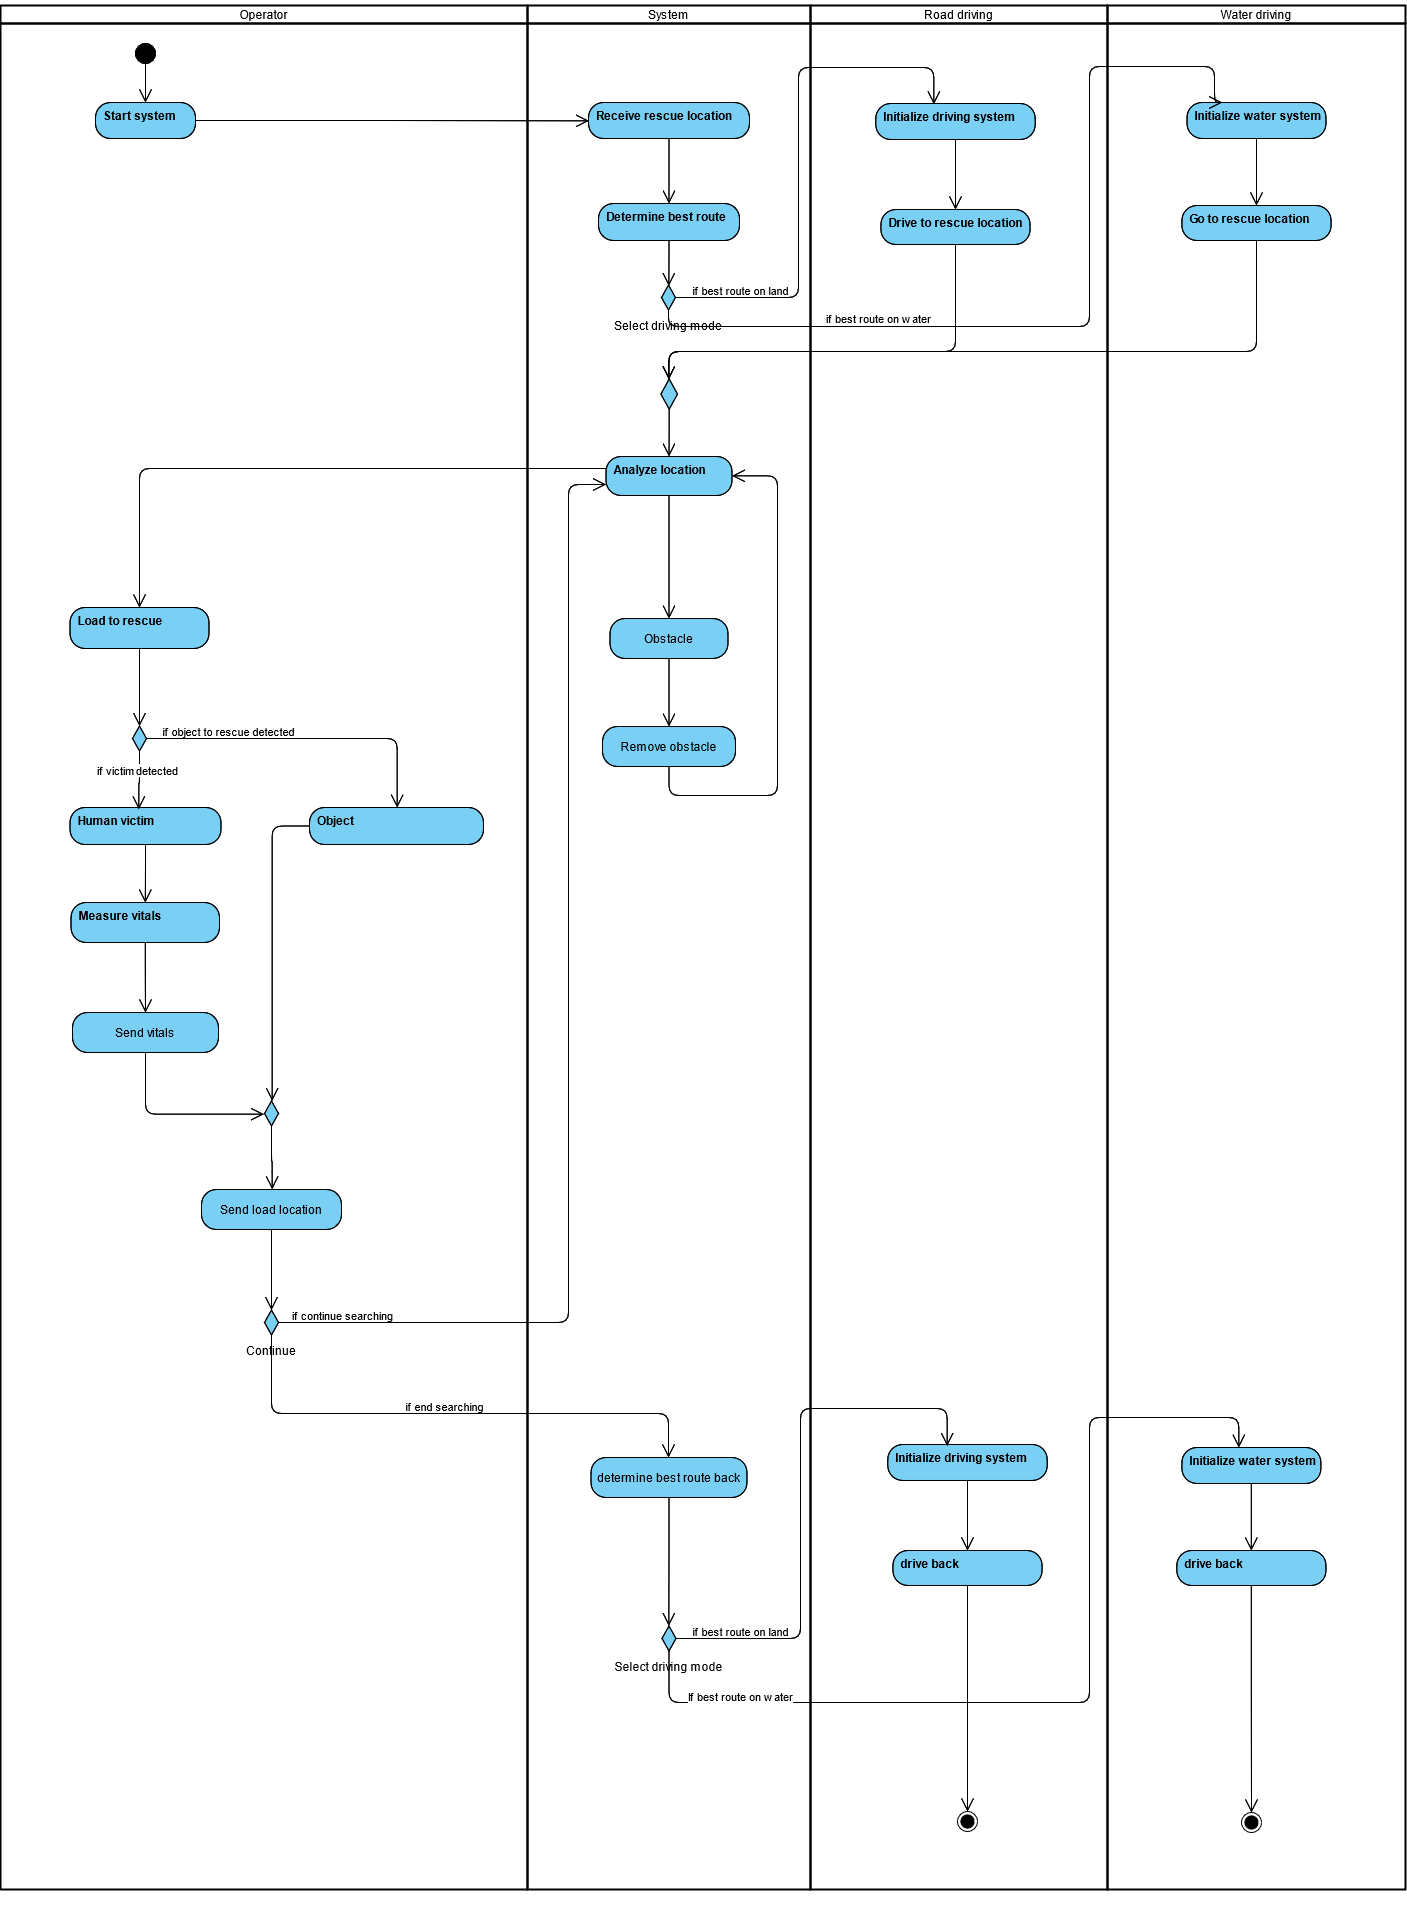
\includegraphics[scale=0.24]{Activity}
\caption{Activity Diagram}
\label{fig:activity}
\end{figure}

The activity diagram presents the actions that will occur in the scenario of the rescue robot system . In the activity diagram , the user starts the rescue robot system and immediately proceeds to the rescue location , determining the possible best routes whether on land or in water.

The Rescue robot system analyses the location and initializes the driving system to drive to the rescue location on how to rescue or remove obstacles, the system will load on objects to rescue after detecting an object whether a human victim or an object.  The same process happens until the end of the search. Fig \ref{fig:activity}

\subsubsection{Use case Diagram}

According to the requirement analysis, the robot rescue system and the victim discovering system are described by the use-case diagram below. The  Rescue robot system comprises sixteen use cases and two actors. The operator actor interacts with the system via the select controlling mode which comprises Automatic, Manual or Hybrid Modes use cases. 

The victim actor interacts with the system through the use case of the Communication and Vital measurements command. This use case also performs command interpretation and calls corresponding use cases to perform the functions. Fig \ref{fig:usecase}

\begin{figure}[h]
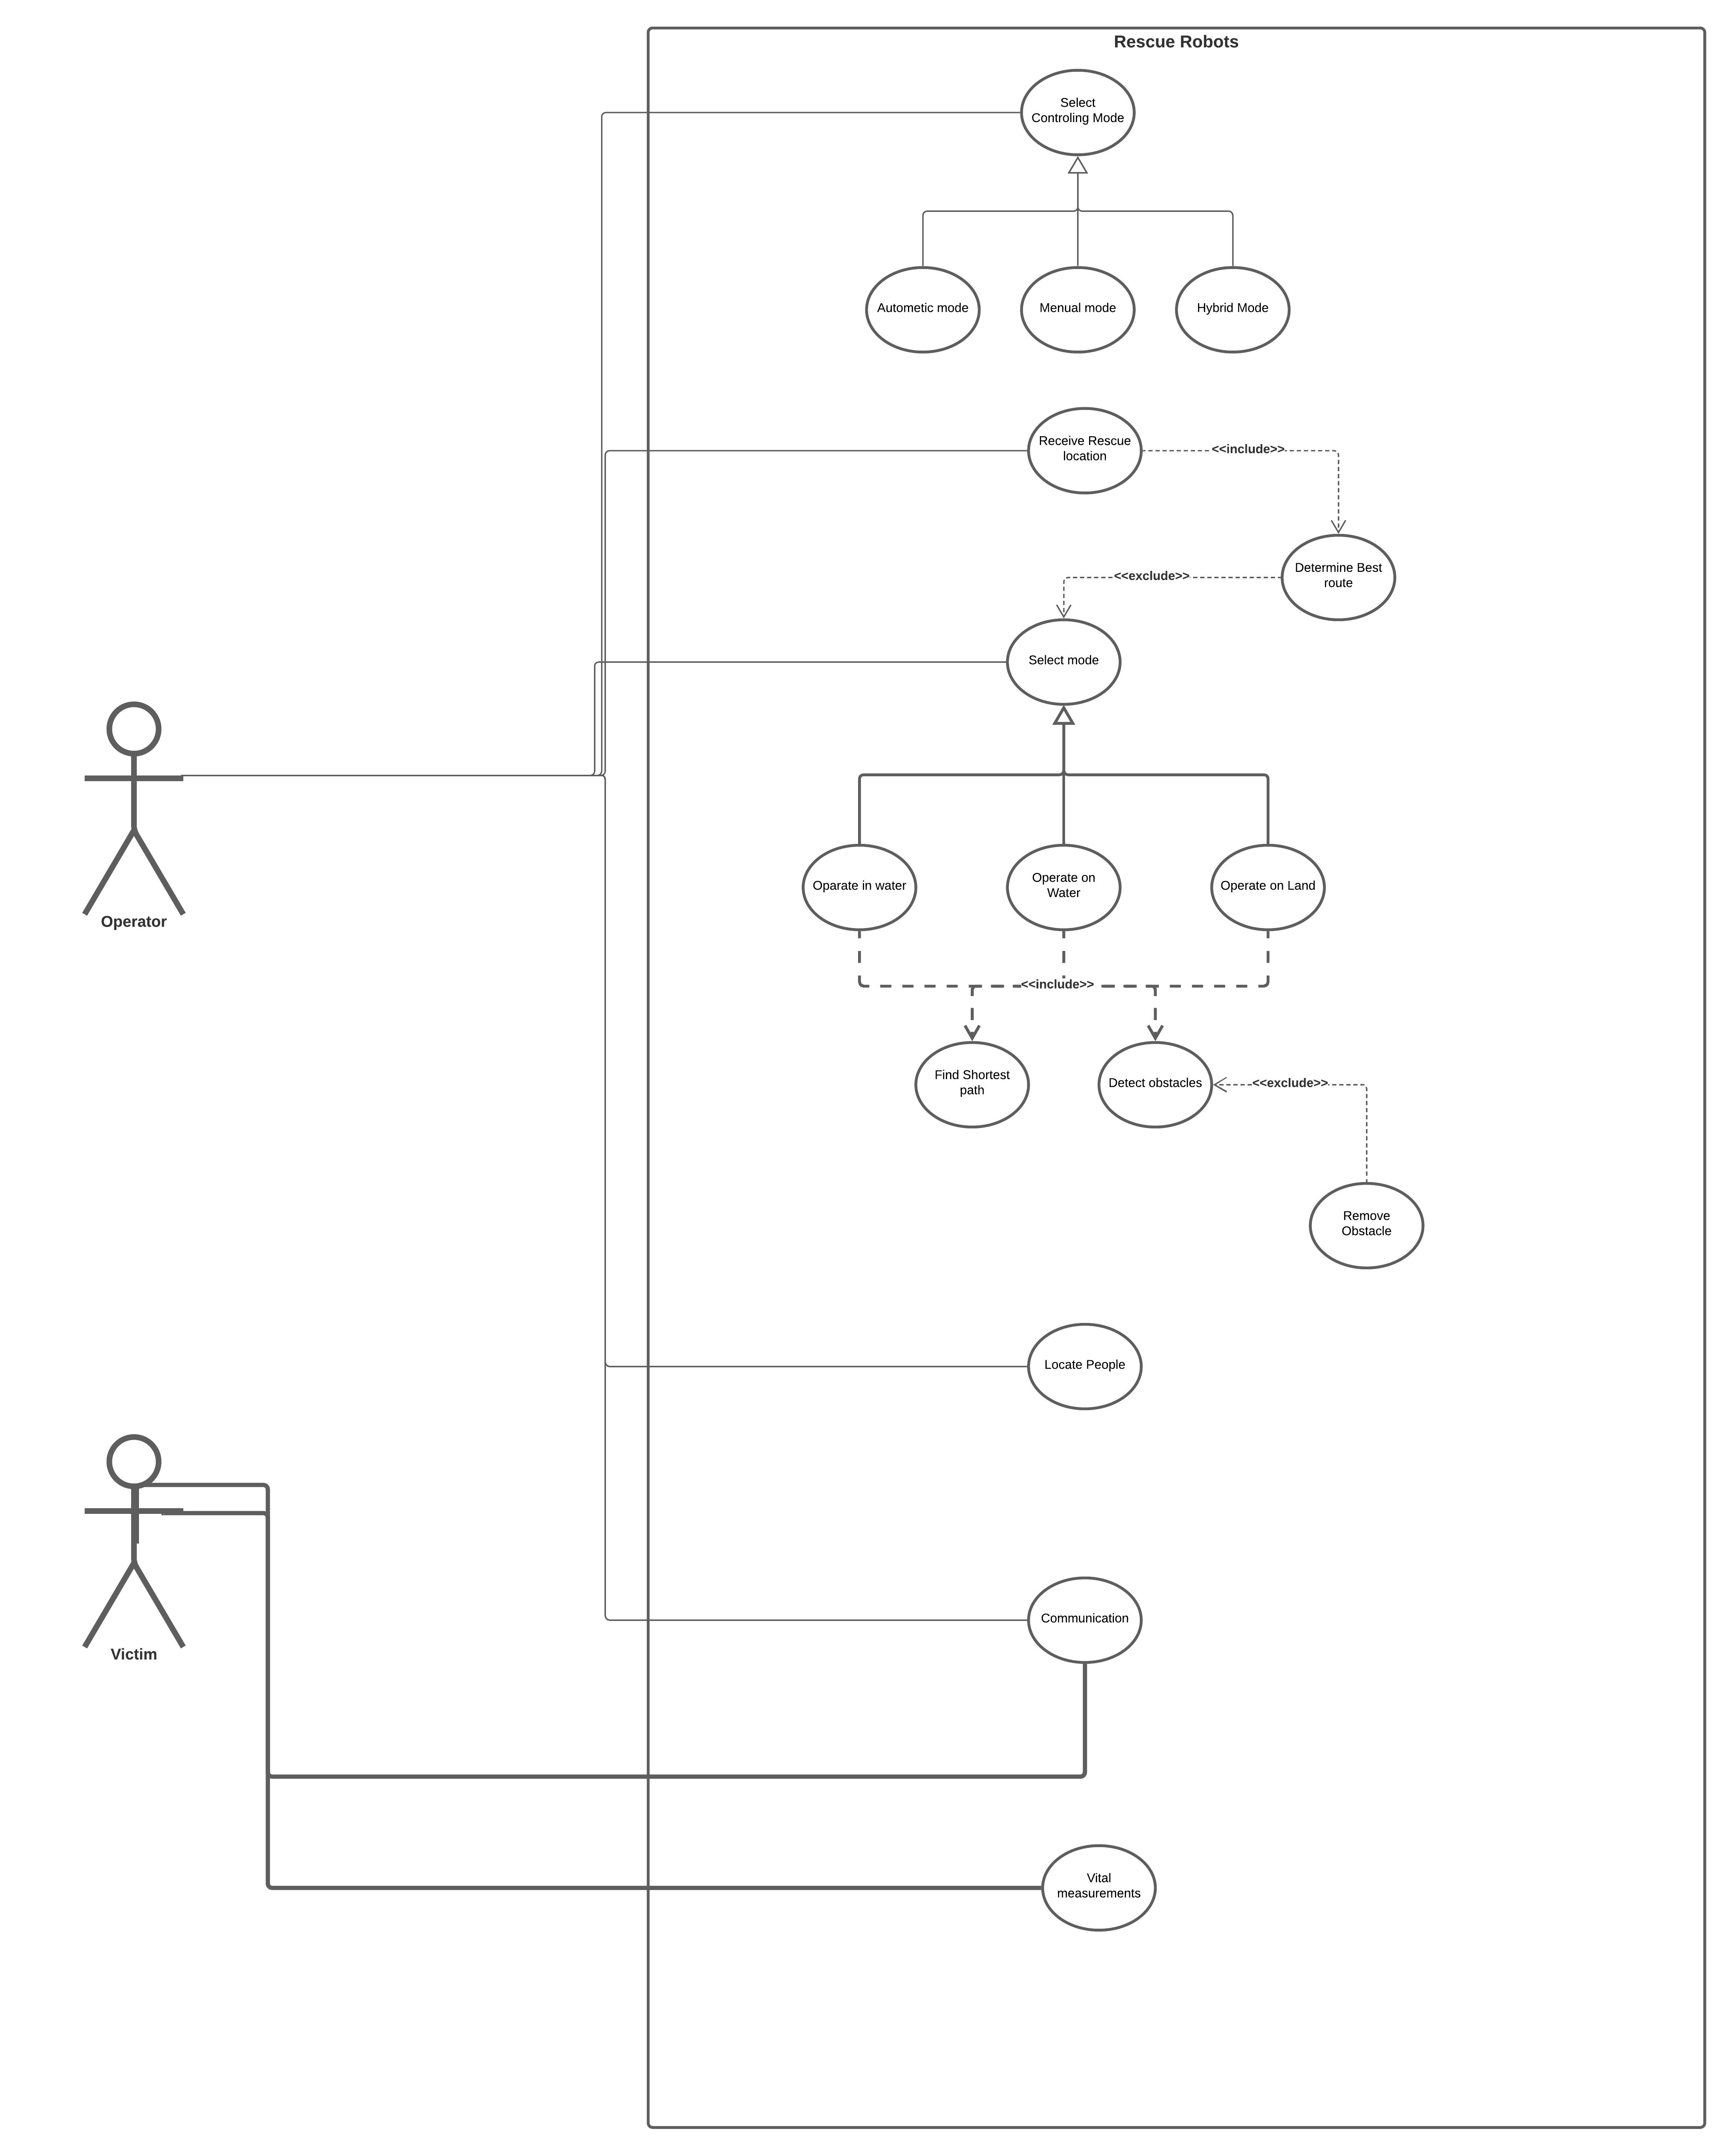
\includegraphics[scale=0.22]{UseCase}
\caption{Use case Diagram}
\label{fig:usecase}
\end{figure}

\subsubsection{Sequence Diagram}

The sequence diagram is used to describe interaction behaviour among the objects and classes in the Rescue robot system. It can also be used to model communications among block structures arranged in time order. 

The diagram below expresses the sequence diagram of the operator and the rescue robot system. When the operator starts the rescue robot system, it sends a command to the system to initialize the driving system for the road/land and water mode. When the connection is established, the system and the rescue robot can communicate and exchange data objects and classes in the system. Fig \ref{fig:sequence}

\begin{figure}[h]
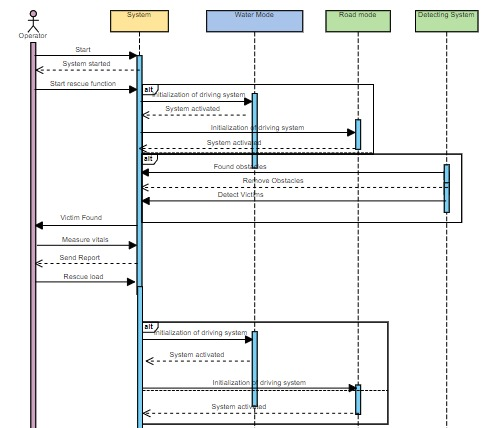
\includegraphics[scale=0.52]{sequence}
\caption{Sequence Diagram}
\label{fig:sequence}
\end{figure}

\subsubsection{State Machine Diagram}

The State Machine Diagram shows us all the states that we can have in our Rescue robot system and the relations or the conditions to go from one state to another. The state machine diagram also represents the behaviour of the Rescue robot system by showing the state of the system in  Operation Method State, Drive Method State, Operation State and Rescue State. Fig \ref{fig:state}

\begin{figure}[h]
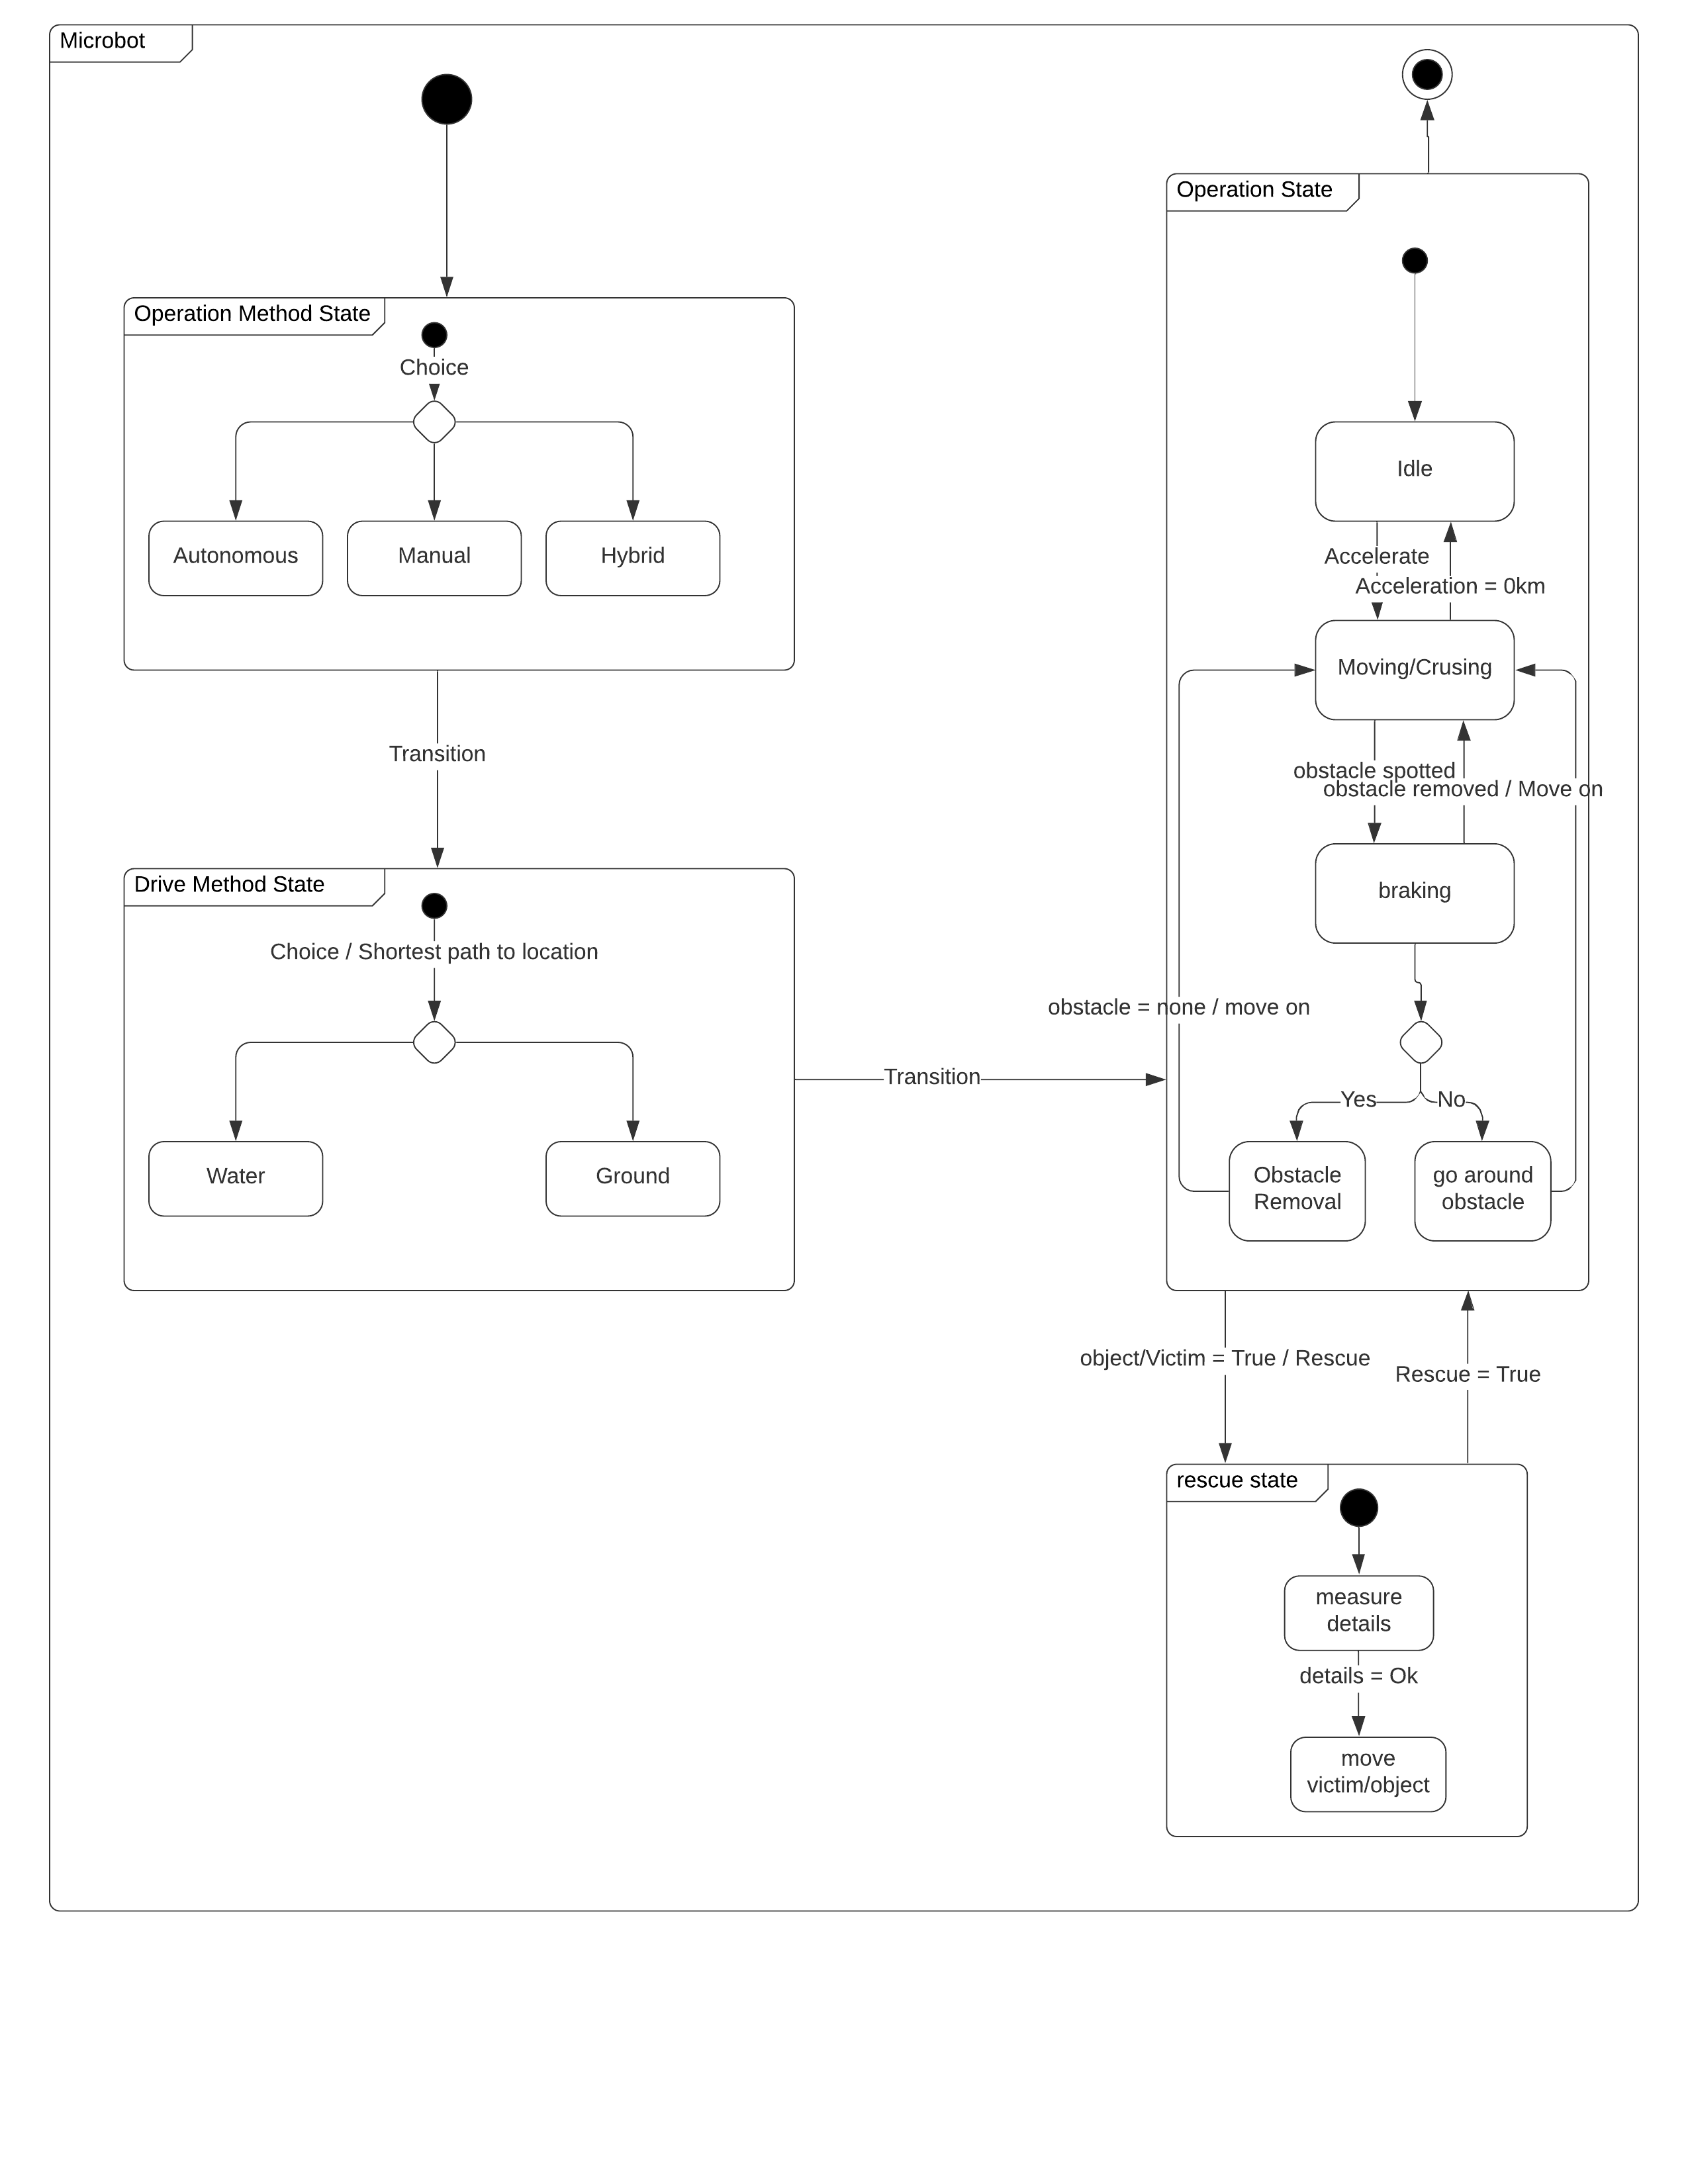
\includegraphics[scale=0.4]{State}
\caption{State Machine Diagram}
\label{fig:state}
\end{figure}

\section{Prototyping (Asadujaman Nur)}

Behind every Great product comes the Design. and a great design defines a great product regarding its looks and functionality, designing the spiderbot took a lot of creative thinking and effort. like the name the robot was made like the shape of Spider. The reason behind it was the way the spider was built. The shape and structure give the spider mobility and flexibility during movement. The same it makes them strong and fierce. And this is what we needed for our robot. Since our robot must operate in unfavourable environment, the design will help us to operate there easily. Our design not only allow our spiderbot to walk on the land, but it also allows it to move on the water as well.

As mentioned on the requirement part our final spiderbot version will be able to do a lot of stuff. But for prototype we decided to spare some of the features, like 360° camera, Biometric sensors, communication devices etc. However, it doesn't make our robot less effective which we discuss later. 

\subsection{Concept Design}

The 360° camera were designed to monitor the surrounding. And an operator could use the camera to project immersive experience while control the robot manually.

\begin{figure}[h]
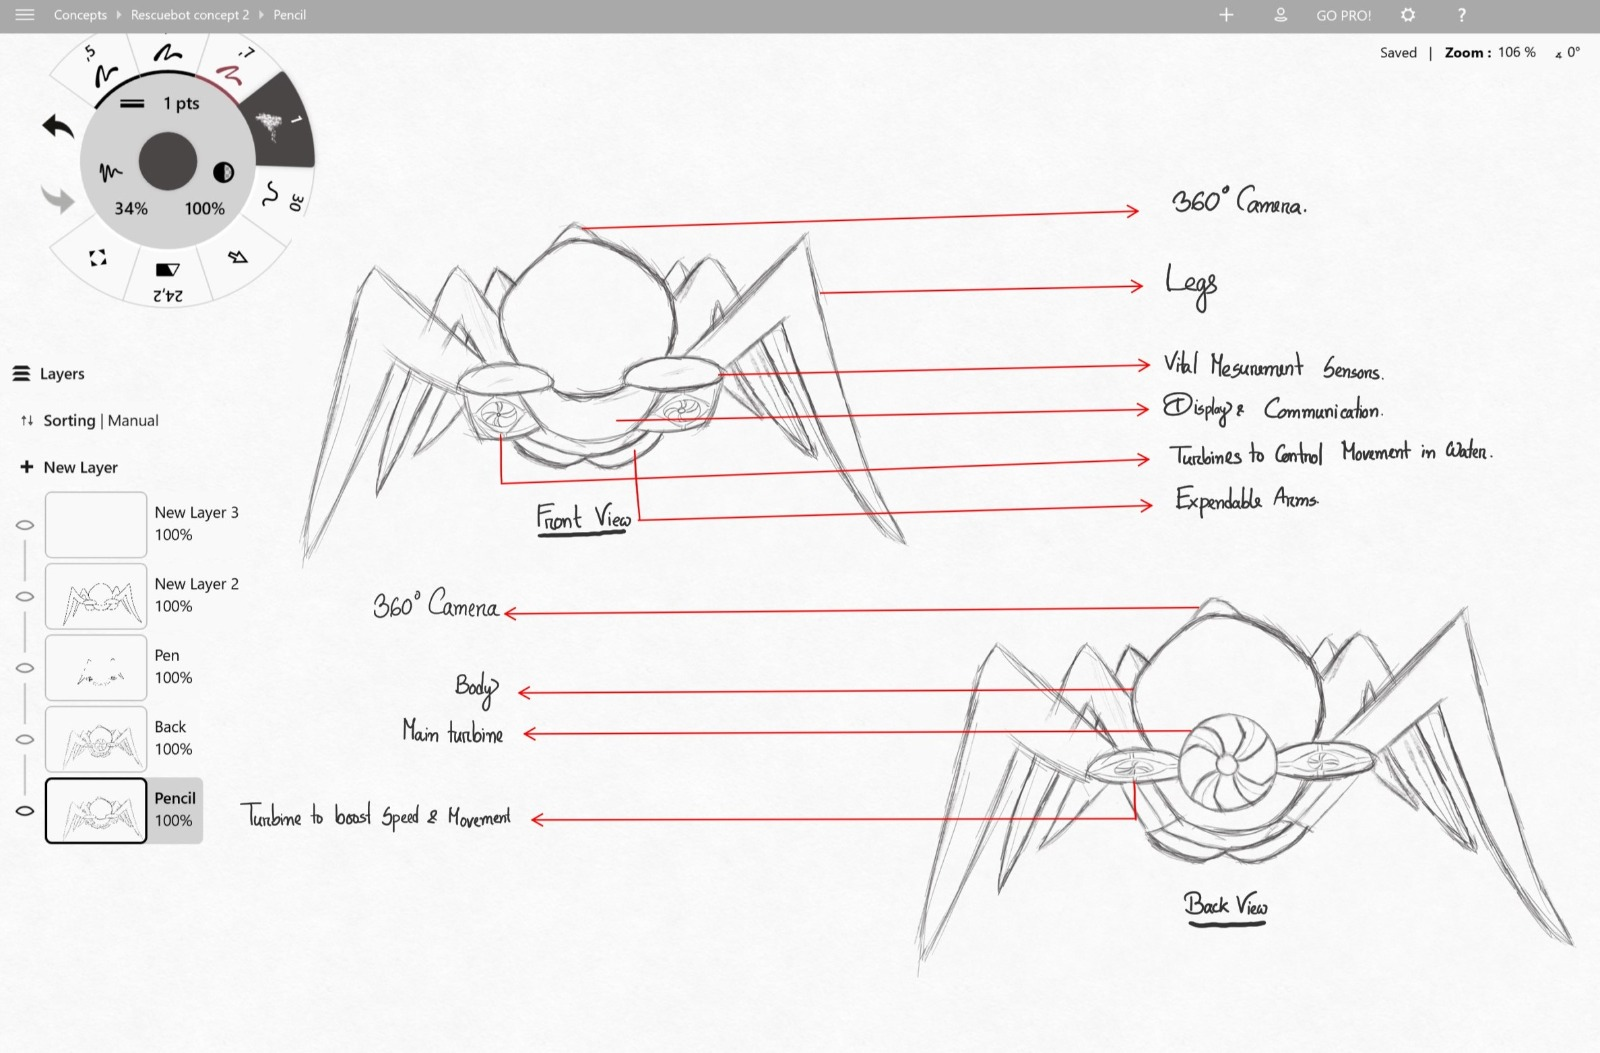
\includegraphics[scale=0.157]{concept}
\caption{Concept Design}
\label{fig:concept}
\end{figure}

Like the spider, our design shares some common features like 6 legs were designed to give maximum efficiency and minimum power consumption while moving.

The front was design to host the vital measurement, display and communication system.

The turbine gives fastest mobility to move on water using water jet technology. The main turbine was design to provide thrust and smaller turbines were designed to provide movement under and on the water.

The arms were design to grasp and push object if necessary.

And the body was designed to chamber most of the electronic components (which we will learn about later) and meant to have some room for emergency supplies like medicine or water while being completely watertight. Fig \ref{fig:concept}

\subsubsection{Changes to the  Design}

As mentioned on the requirement part our final spiderbot version will be able to do a lot of stuff. But for prototype we decided to remove and add some of the features, like 360° camera, Biometric sensors, communication devices, the arm and small turbines and ability to dive under water were removed. However, a boat shape body were added to provide the ability to float, and a different control method were added to control the movement on the water.

Later, we will only talk about the features that we are implementing on the prototype not the final version of our spiderbot.

\begin{figure}[h]
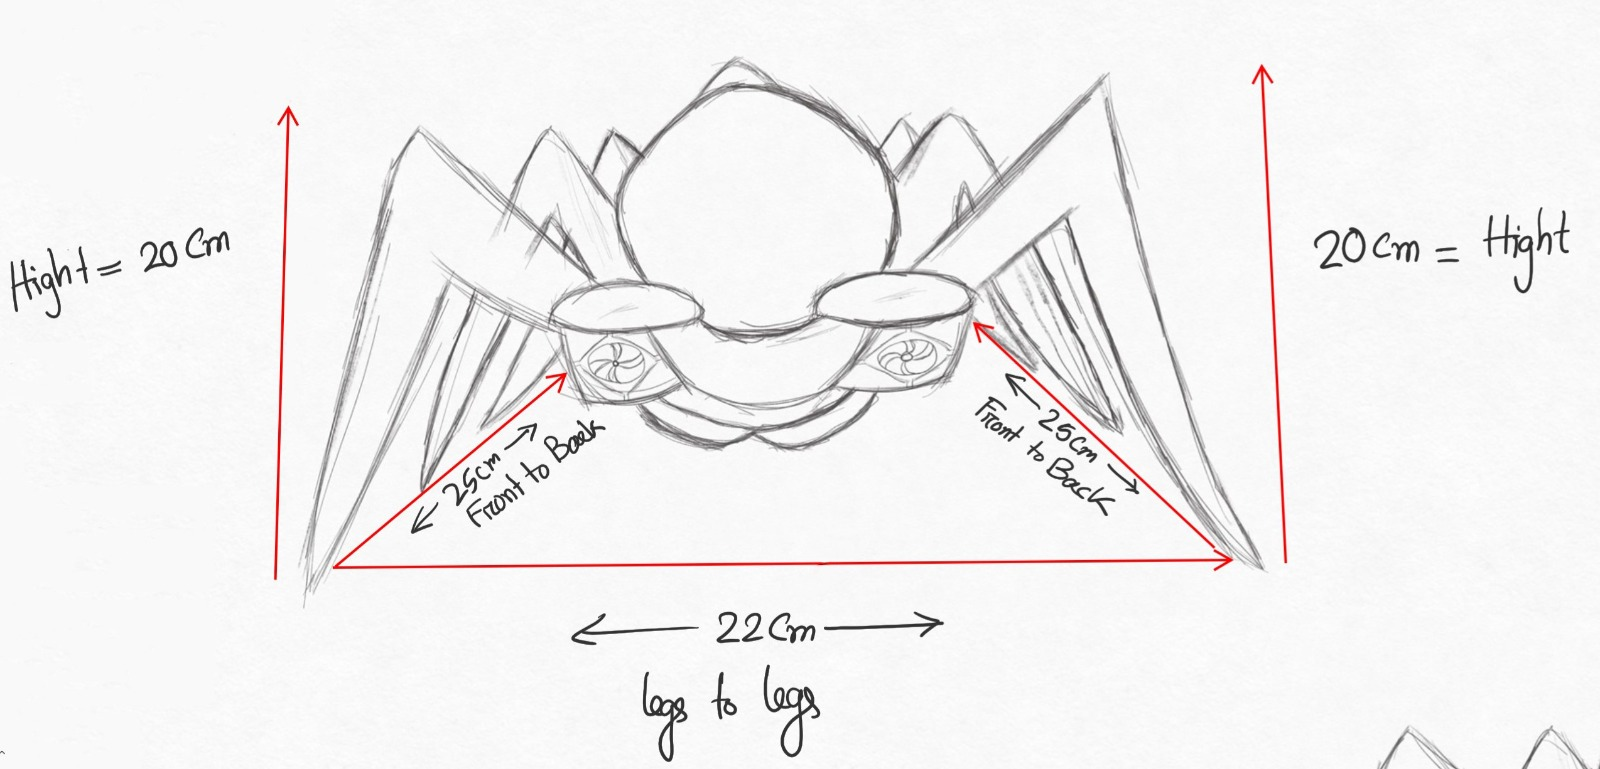
\includegraphics[scale=0.158]{spidermodel}
\caption{Spider bot dimensions}
\label{fig:spidermodel}
\end{figure}

\subsection{3D MODELING}

To Make 3d model of our spiderbot we took the help of solid works. And this is the rough sketch we followed to make our model.

We followed the dimension for the overall size of our spiderbot and we followed the 1:10 requirement for the 3D modelling. Fig \ref{fig:spidermodel}

And for the individual part this dimension was followed. Just to mention the arm was the finial part we decided to remove. But we are going to leave the arm here so that gives a better contrast on the dimension idea.

\subsubsection{Legs}

Following the design, we were able to recreate the 3D model in SolidWorks. Fig \ref{fig:legs}.

\begin{figure}[h]
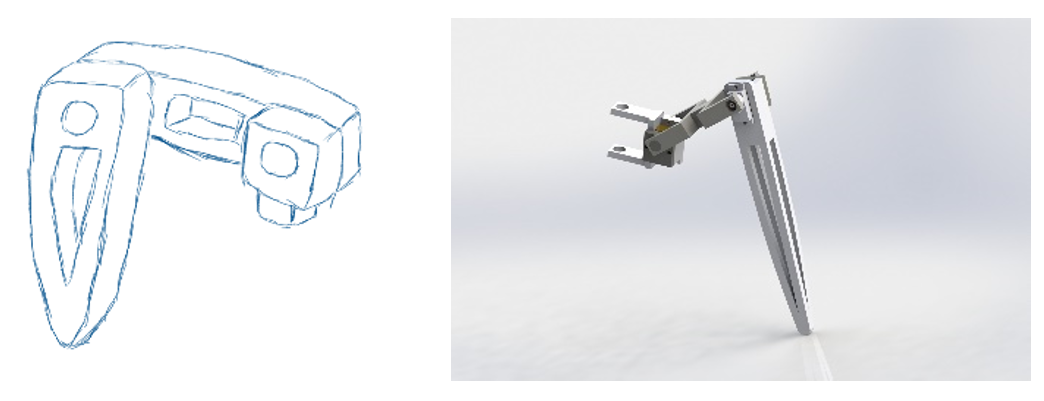
\includegraphics[scale=0.34]{legs}
\caption{Legs}
\label{fig:legs}
\end{figure}

\subsubsection{Body/Chassis}

The main body and the chassis is the center point of the SpiderBot. It was designed in such a way, so that it can host most of the electronic components and the body acts as a protective shield for the environment. Like we mentioned earlier, some parts were added, the par like boat shape is the part has been added to give the spiderbot the ability to flow through water. Fig \ref{fig:body}.

\begin{figure}[h]
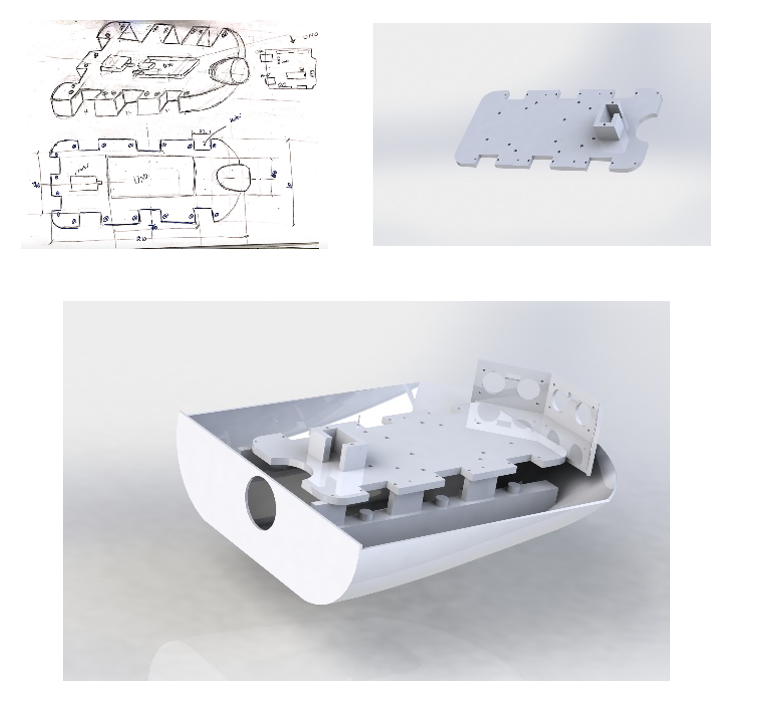
\includegraphics[scale=0.48]{bodychasis}
\caption{Body/Chassis}
\label{fig:body}
\end{figure}

\subsubsection{Turbine}

The same principals were followed to design and 3D model to create the turbine. Later, it was attached to the body. So, it prevents water from coming inside, thus water-sealed. Fig \ref{fig:turbine}.

\begin{figure}[h]
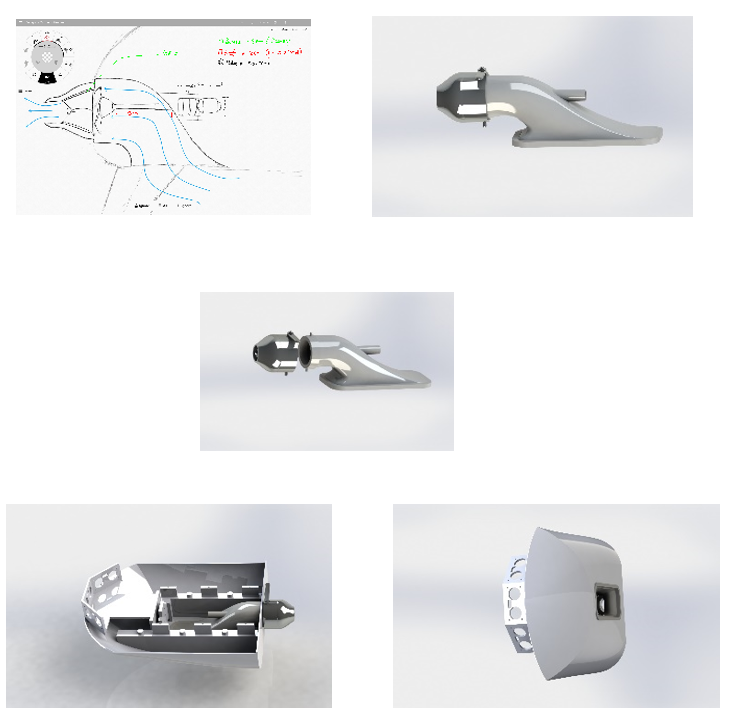
\includegraphics[scale=0.47]{turbine}
\caption{Turbine}
\label{fig:turbine}
\end{figure}

\subsubsection{Final Model for prototype}

So, finally with some addition and subtraction the final version of our spiderbot will look like the picture above. Here we have 3 different views from different perspective. Fig \ref{fig:finalmodel}.

\begin{figure}[h]
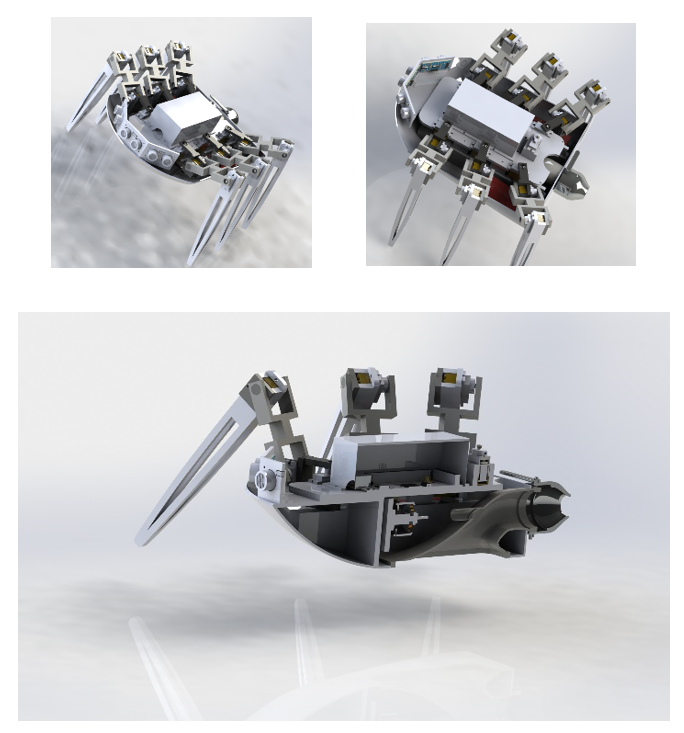
\includegraphics[scale=0.49]{finalmodel}
\caption{Final Model for prototype}
\label{fig:finalmodel}
\end{figure}

\subsection{Materials}

One of the biggest aspects of designing is to choose the right materials for the product. Therefore, to 3D print our spider bot prototype, our primary choice of material is plastic however for the final version of our spiderbot we will use different materials based one the body parts. for example:

For the body, our primary choice is mixture of carbon fiber and Stainless steel which will provide strength and durability to our robot.

However, to add grip on the legs some rubber tip will be added on the tip of the legs. Thus, it will act like shoes for the robot and like the shoes it will be easy to replace therefore it will add extra protection as well as easy maintainability.

\subsection{Tools}
To help us archive the great design for our spiderbot some tools were used.
The list of these tools will be mentioned below.

•	Concepts: a drawing software which was used to design the concept for spiderbot.

•	SolidWorks was used to build our 3D prototype.

•	CURA was used to do measurements for 3D printing.

By combining the tools and all the skills we have spiderbot came to live from our imagination.
 

\section{Electronic Design (Abeeb Nureni)}

\subsection{CONSTITUENTS OF THE RESCUBOT}

This is a major stage of the design implementation, the robot will not be able to do anything if the essential parts/components have not been considered and for this reason we have carefully put together the right components, selection made with good ratings to suit the project specification such that the robot can autonomously or manually be controlled while working on land or sailing through the water and this is what has been covered in the project write-up.

Since the robot must operate on land and water, thereby making the design to take into consideration the two main parts for its locomotion which are legs for land and flap for water. Below is the description of the selected electronics components for the robotic operation during the project.

\subsubsection{Arduino mega2560 microcontroller}

This is the main building block for the robot, it has 54 channels which can conveniently handle several analogue inputs/outputs which could either actuators (servo motor) or transducer(sensors). The microcontroller gets the programmed codes from the computer using USB cable with other hardware connected to it and the robot can perform according to the specifications. \cite{mega} Fig \ref{fig:mega}

\begin{figure}[h]
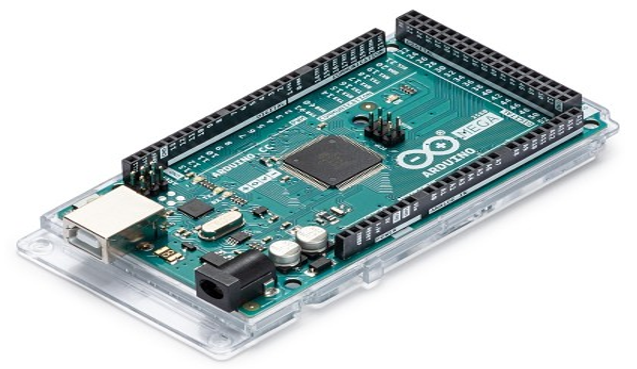
\includegraphics[scale=0.51]{mega}
\caption{Arduino mega2560 microcontroller}
\label{fig:mega}
\end{figure}

\subsubsection{Servo Motors}

It is important for the rotary parts of the robot legs to have high precision as it will move in all directions and the ability to respond fast to any change in the direction is the reason for the choice of servo motor. The robot has six legs and each of the legs has been designed to have three supportive, rotary, and flexible joints; the joints provide the robot the ability to manoeuvre over the obstacles. Each of the joints is used by the robot with the help of the servo motor that is fixed to this joint on the robot. The degree of freedom of these legs are not limited and with better precision. \cite{robarm} Fig \ref{fig:servo}.

\begin{figure}[h]
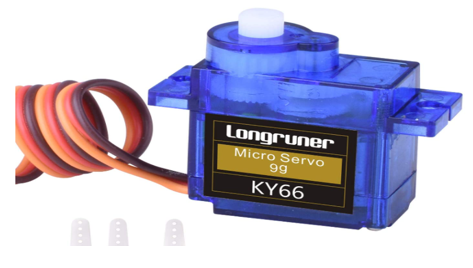
\includegraphics[scale=0.72]{servo}
\caption{Servo Motors}
\label{fig:servo}
\end{figure}


\subsubsection{Ultra-sonic Sensor}

According to the specification of the project, the robot needs to sense an obstacle and overcome or manoeuvre over the obstacle, choose the best route, hence the need for a sensor which serves as the eyes of the robot and can assist the robot to sense the obstacles and decide to overcome them. The ultrasonic sensor consists of a transmitter and a receiver. The transmitter transmits an ultrasonic sounds within an acceptable range of the component usually between 20KHz - 200KHz which is greater than that of human hearing and the receiver is used to detect the response which is in form of pulses and then used by the system to process its signal .These signals are used by the robot in terms of which direction it want to move either to avoid obstacle or move through the fastest route as this process is covered in the coding part of the project \cite{ultrasonic} Fig \ref{fig:ultrasonic}.


\begin{figure}[h]
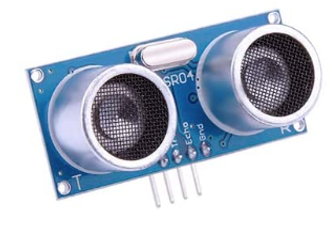
\includegraphics[scale=0.80]{ultrasonic}
\caption{Ultra-sonic Sensor}
\label{fig:ultrasonic}
\end{figure}

\subsubsection{Power Supply}

To make the robot to work, it must be connected to a source of power and the most efficient source of robotic power is the use of a DC batteries which comes in various sizes, rating, and design. The selected battery for our robot is based on the calculated energy of the adjoining parts such as servo motor, sensor, turbine fan etc. and taking into consideration the cost and effect of weight on the overall system. The prototype of the robot falls under the category of a small machine thereby require less power, hence the choice of a DC battery. Furthermore, most microcontrollers operate between 9 - 12V with an Arduino having a 5V regulator; the actuators (servomotors) used operates between 6 - 9V and finally Transducers (sensors) use 5V. A table is presented below for all the component required and their respective specifications which helped in arriving at the calculated rating of the battery, hence our decision for a pair of battery Fig \ref{fig:battery}.

\begin{figure}[h]
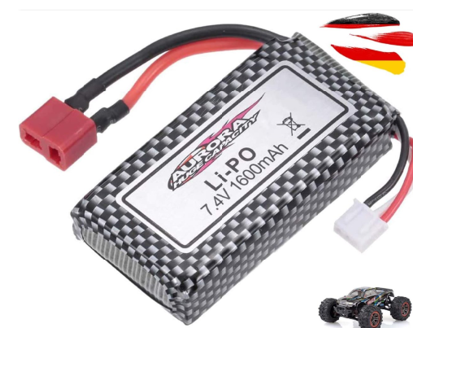
\includegraphics[scale=0.80]{battery}
\caption{DC Battery}
\label{fig:battery}
\end{figure}

\subsubsection{Turbine}

The operation of our robot in water can be achieved by using a turbine, the turbine would have a blade, shaft and a motor which are responsible for the driving of robot on water. The motor drives the blade with shaft connected to it and turn clockwise or anti-clockwise depending on if the robot wants to move forward or backward and this creates the required up-thrust for the robot to move in water. The size and the rating of the turbine used was carefully selected to reduce weight and improve efficiency. Fig \ref{fig:motturbine}.


\begin{figure}[h]
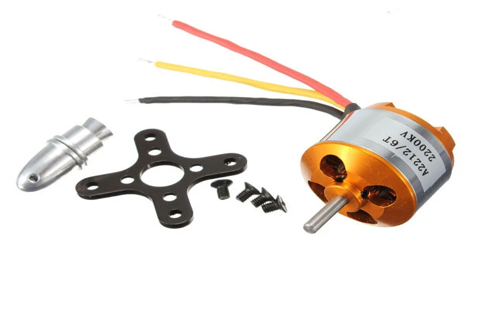
\includegraphics[scale=0.73]{motturbine}
\caption{Turbine}
\label{fig:motturbine}
\end{figure}

\subsection{Control Techniques}

The robot upon its completion could be controlled in two ways which are by control pad and by computer. When using a control pad, the operator will be able to control the robot and they will both stay in proximity. Use of joystick make it easier for the operator to navigate the robot in all directions. The robot could also work autonomously, and the control is done by computer, which is stationed in a control room, the activities of the robot can be monitored and controlled remotely. Depending on what the situation is either of the two methods can be employed to control the robot. These control methods would work perfectly with the implemented codes which is in C language which is later presented in this paper. Fig \ref{fig:wireless}.


\begin{figure}[h]
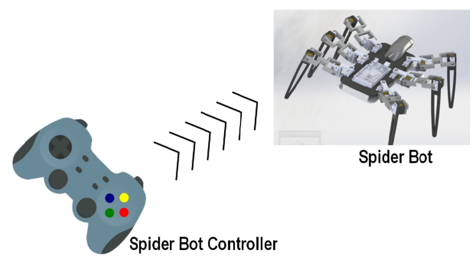
\includegraphics[scale=0.73]{wireless}
\caption{Robot Controller}
\label{fig:wireless}
\end{figure}

To have a grasp of how the electronic components are placed on the robot, the anatomy of the robot is shown in Fig \ref{fig:anatomy}.



\begin{figure}[h]
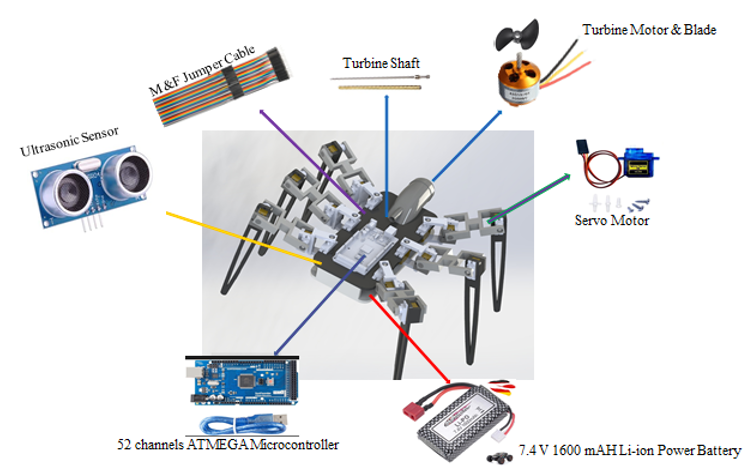
\includegraphics[scale=0.48]{anatomy}
\caption{Anatomy of the Rescubot}
\label{fig:anatomy}
\end{figure}


\subsection{Components}

The table below shows our chosen electronic components and their specifications Table \ref{componetlist}. \cite{conrad}

\begin{table}[ht]
\centering
\begin{tabular}{|c|c|c|}
\hline
S/N & Item & Quantities  \\ 
\hline
\hline
1 & ATmega2560 Microcontroller 52 channels & 1 \\
2 & 7.4 V 1600 mAh Li-ion Power Battery & 2 \\
3 & Adafruit Motor Micro Servo - MG90S  & 21  \\
4 & Breadboard Jumper Wires  & 1  \\
5 & Soldering Strips Grid Board & 4  \\
6 & HC-SR04 Ultrasonic Module Distance Sensor & 3  \\
7 & Electrical Insulation Tape &  1 \\
8 & Turbine Motor &  1 \\
9 & Turbine Shaft( 8mm / 4mm ) 13 cm &  1 \\
10 & Turbine Blade &  1 \\
11 & Joystick with JST-HX254 Stecker & 2 \\
12 & Arduino AG MKR CAN SHIELD &  1 \\
13 & Arduino Board NANO RP2040  &  1 \\
14 & Resistor kit &  1 \\
15 & 1000 uF 16 V &  16 \\
16 & 7.4V block battery alkaline manganese  &  2 \\
17 & Beltrona 9V-I-Clip Batterieclip 1x 7.4V Block  &  2 \\
\hline
\end{tabular}
\caption{Componet list}
\label{componetlist}
\end{table}




\section{Prototyping Programming (Marwa Hassan)}

During the programming and simulation phases, the robot starts to develop its own view of the world using  few symbols to represent each object, we have been  asked to deal with different environments and program the robot to reach its target.
In the next section, we are going to explain how we dealt with each required task, so that we end up having a robot that meet all the requirements. We have developed our code functions in C using Visual Studio Code tool. 


\subsection{Different Targets}

Throughout the  representation of  the Robot's world by a single map defined with character  array, the Robot was defined by character 'R', and asked to  reach either a land target defined by  'T' or sea target 't', and return to its home base which defined by ‘X’ after the robot leaves the initial position taking into consideration that, after the robot pick its  target the position will  turn into ‘O’ and the robot has a limitation of  maximum 200 steps. 


\begin{figure}[!h]
	
	\centering
	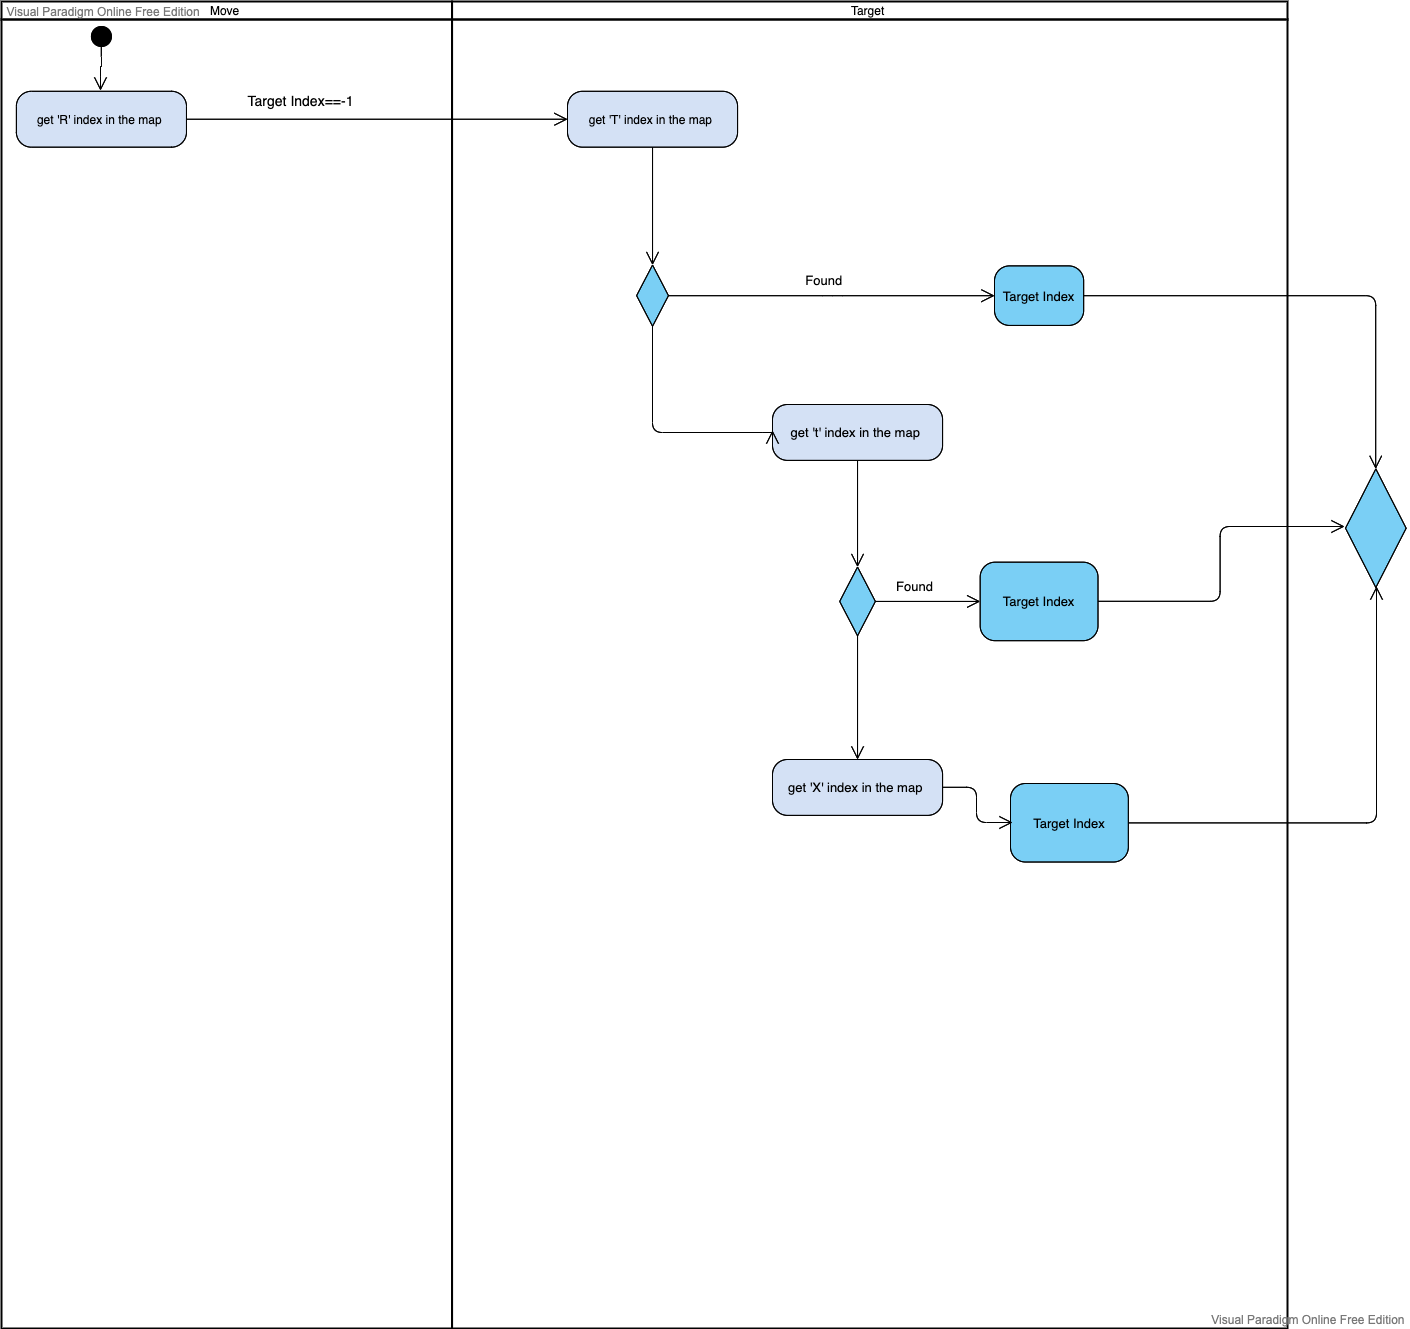
\includegraphics[width=0.4\textwidth]{targets.png}
	\caption{\label{targetAct}Different Target's Activity Diagram }
	
\end{figure}

The Fig.\ref{targetAct}   shows the activity diagram of our  approach we used to deal with different Targets.


Our approach to solve this challenge, was to initialize a Target index by "-1" after getting the Robot index in the map, the function"get\_pos" start to search for first the target 'T' if found it will then consider it as the current Target index, if  not then as next step it searches for target 't' and considered it as current target index, as a third step the function will search for the target 'X' which is the home base and considered it as the current target. Fig. \ref{targetCode}shows  the code implementation of this task. 

\begin{figure}[!h]
	
	\centering
	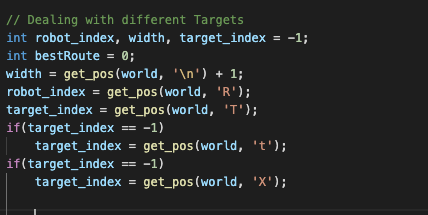
\includegraphics[width=0.4\textwidth]{targetsCode.png}
	\caption{\label{targetCode}Targets code.}
	
\end{figure}

\subsection{Avoiding Walls }

As a next task, the robot were asked to avoid crashing into walls, which is represented by '\#' , to develop that, a function ' move ' should return  an integer that represents the direction, where the robot should navigate as follows : for  North return 1,  East return 2,  South return  3
and West return  4, the Fig .\ref{wallAct} shows the activity diagram of our approach to avoid the wall.


\begin{figure}[!h]
	\centering
	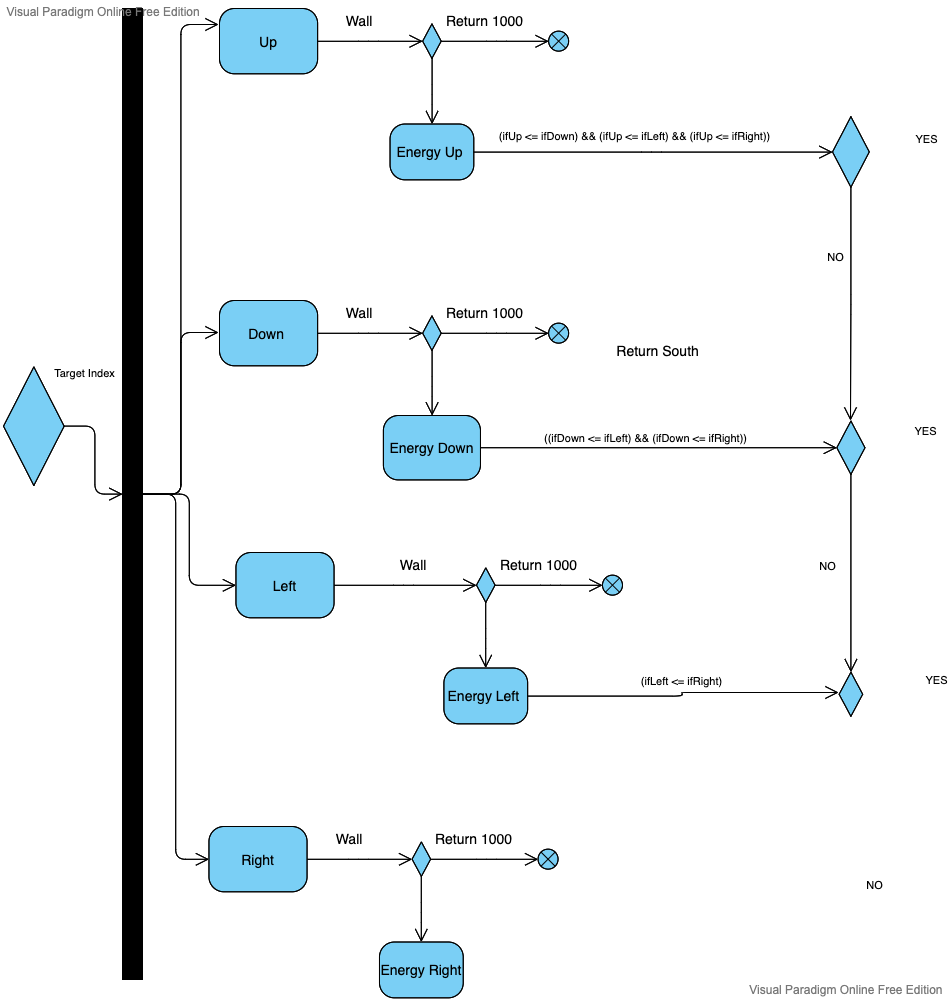
\includegraphics[width=0.4\textwidth]{wall.png}
	\caption{\label{wallAct}Avoiding walls  Activity Diagram }
	
\end{figure}


Our approach to solve this challenge, was to get  Min. steps in each direction by passing the next step to function called "minEnergy" and returning the value and store it in four variable "ifUp indicate North direction ", "ifDown for South direction ", "ifRight for East " and "IfLeft for West". The Fig.\ref{MinEnAct}shows  the activity diagram of the "minEnergy " Function. 

\begin{figure}[!h]
	
	\centering
	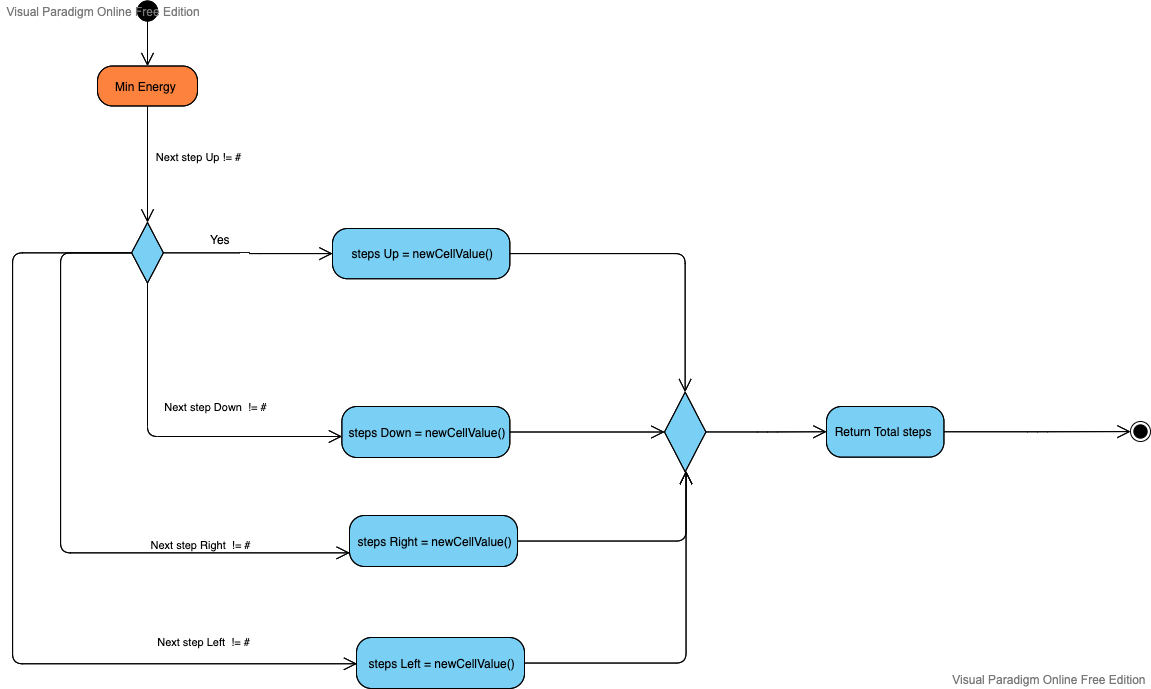
\includegraphics[width=0.4\textwidth]{MinEnergy.png}
	\caption{\label{MinEnAct}min.Energy Activity Diagram .}
	
\end{figure}



The minEnergy function check if the next potential step is wall, it will return then a '1000' which can be considered as great value, so the robot won't ever consider this direction, or the other option is that it returns the actual number of steps when taking this direction, the Fig \ref{MinEnCode} shows the code implementation of minEnergy function.


\begin{figure}[!h]
	
	\centering
	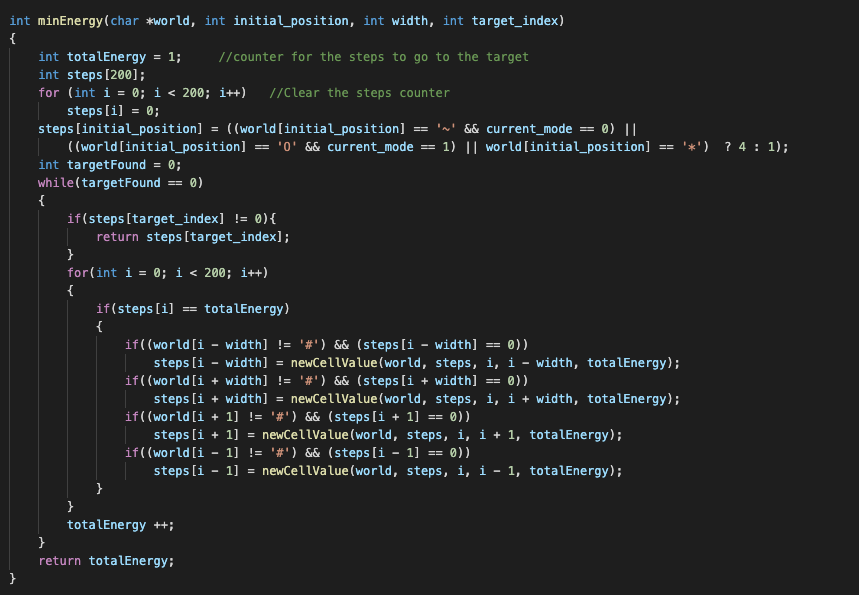
\includegraphics[width=0.4\textwidth]{MinEnergyCode.png}
	\caption{\label{MinEnCode}The implementation of minEnergy function  .}
	
\end{figure}

After the calculation  of the potential value in each direction, the values are get compared  and store in variable called "bestRoute" which hold one of the direction NORTH, SOUTH, EAST and WEST and considered it as the best route to reach the target, Fig \ref{MinstepsCode} shows the implementation of this step. 


\begin{figure}[!h]
	
	\centering
	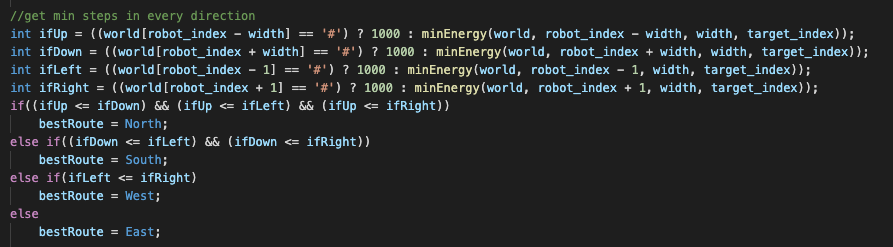
\includegraphics[width=0.4\textwidth]{minStepsCode.png}
	\caption{\label{MinstepsCode}The implementation of bestRoute  .}
	
\end{figure}



\subsection{Water Mode }


One of the Robot requirement is the ability to drive on water, which represented by  ($\sim$) symbol . To drive through water, the Robot should have to  toggle from Land to Water Mode and vice versa.  In addition to returning  1,2,3,4 to the directions  the robot should return 5 in the
move function to toggle the driving mode, the Fig.\ref{ToggleAct} shows our Approach to switch between the Two modes. 


\begin{figure}[!h]
	
	\centering
	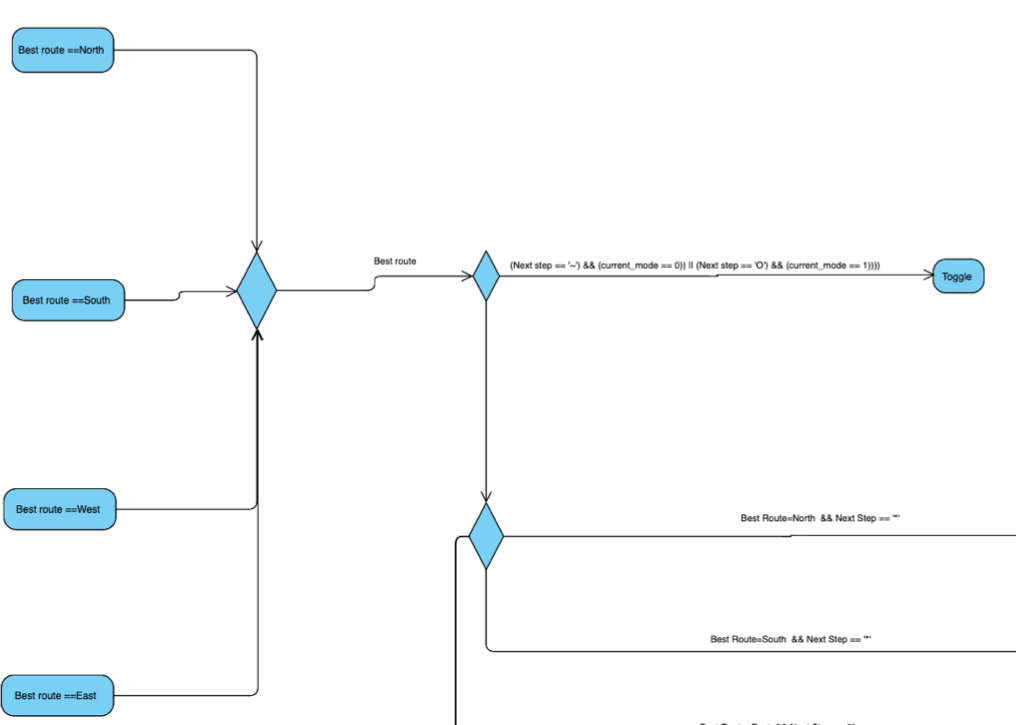
\includegraphics[width=0.4\textwidth]{Toggle.png}
	\caption{\label{ToggleAct}Activity diagram of Toggle scenario  .}
	
\end{figure}


After the best route is defined, the move function check if the next step is water and the current mode is Land, and return a Toggle. As well as checking the other scenario if the next step is land and the current mode is water, it will toggle the mode. The Fig.\ref{ToggleCode} shows the code implementation of this task.


\begin{figure}[!h]
	
	\centering
	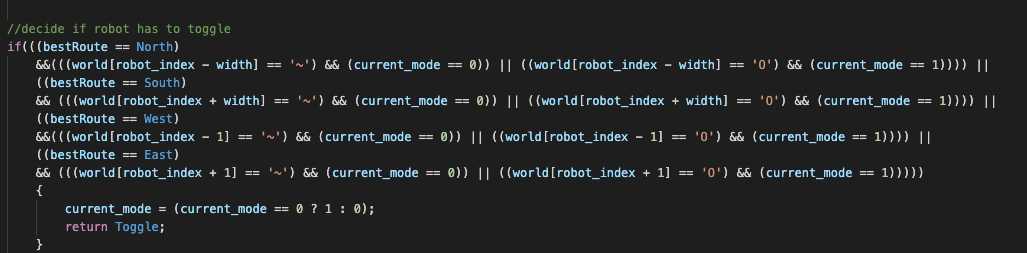
\includegraphics[width=0.4\textwidth]{ToggleCode.png}
	\caption{\label{ToggleCode}The implementation of Toggle scenario  .}
	
\end{figure}


\subsection{ Dealing with Obstacles}

As a last Task the Robot's world gets more complicated to consider new barriers, beside the Wall the map will contain  obstacles described with  (‘*’) symbol, that can be destroyed, The robot will consume  energy based on  10 unit energy per movement,  30 unit energy per toggle and  70 unit energy for trying to destroy an obstacle, and we will have to use min Energy to fulfill the task. 

In addition, if we choose to destroy the  obstacle, the function will return a new value as  6 to  destroy an obstacle to the north, 7 to destroy an obstacle to the east,8 to destroy an obstacle to the south and  9 to destroy an obstacle to the west. The Fig. \ref{ObstAct} shows our approach to solve this task .

\begin{figure}[!h]
	
	\centering
	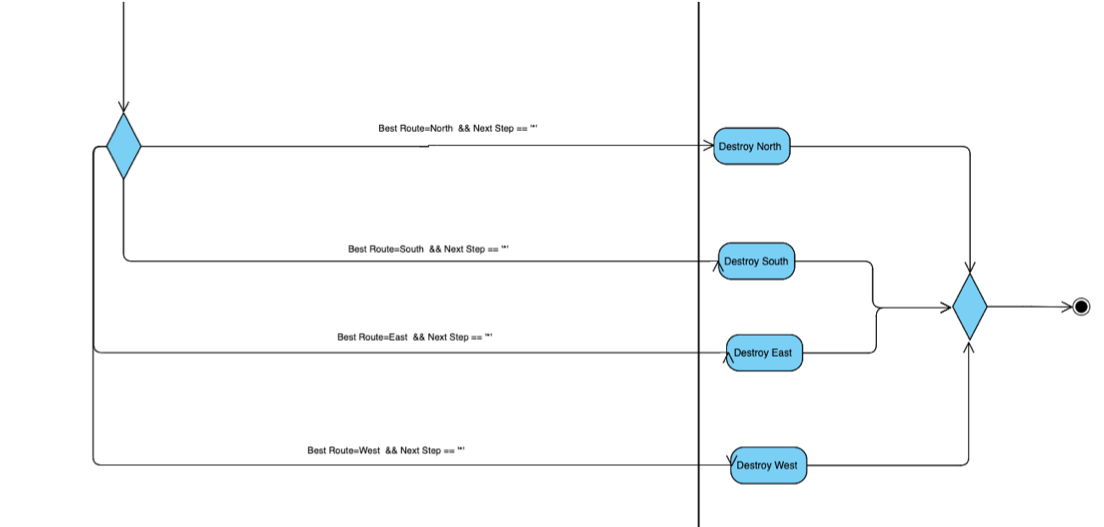
\includegraphics[width=0.4\textwidth]{Obstecles.png}
	\caption{\label{ObstAct}Activity diagram of dealing with obstecles  .}
	
\end{figure}


After getting the best route, the function newCellValue will return either Energy+ 1, when they meet any Target, or Energy+4, if  it faces any Obstacle in any direction or if faces a water or land, when need to toggle. The fact that it will return only 4 when destroying an obstacle, because the robot will consume only one time the amount of energy to destroy the obstacles in  the two-way path. The Fig.   \ref{nextstepAct} shows the activity diagram of newCellValue and how it returns either Energy+1 or Energy+4. 

\begin{figure}[!h]
	
	\centering
	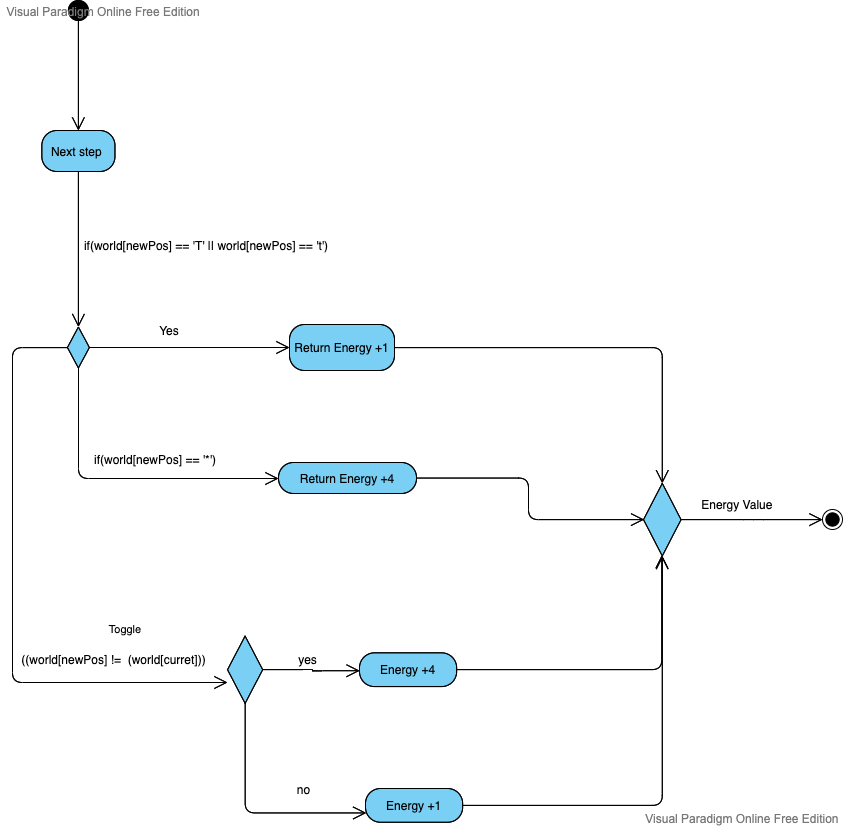
\includegraphics[width=0.4\textwidth]{NextStep.png}
	\caption{\label{nextstepAct}Activity diagram of newcellValue function .}
	
\end{figure}



The implementation of the function is shown in Fig. \ref{calCode}


\begin{figure}[!h]
	
	\centering
	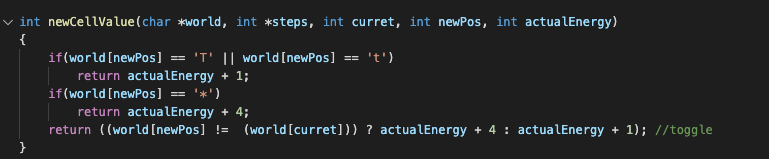
\includegraphics[width=0.5\textwidth]{newCalCode.png}
	\caption{\label{calCode} Implementation of newcellValue function .}
	
\end{figure}


After getting the best route and the potential next step contains any obstacle, the function  will then return to destroy in this direction to deal with the obstacle. The checking of conditions is done in four direction North, South, East, west, If the robot's best route doesn't contain any obstacles, it will send then the best Route. The Fig. \ref{obstCode} shows the code implementation when destroying obstacle. 

\begin{figure}[!h]
	
	\centering
	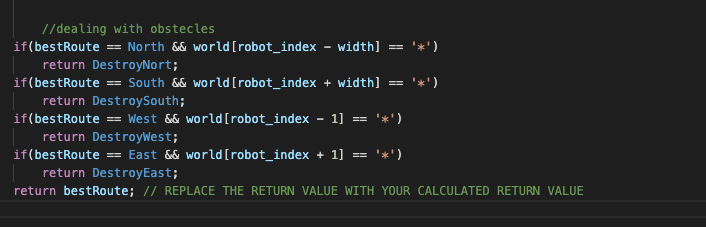
\includegraphics[width=0.4\textwidth]{oBSTECLEScODE.png}
	\caption{\label{obstCode} Implementation of destroying obstacles scenario  .}
	
\end{figure}



\section{Header file (Miguel Rodriguez)}


\begin{lstlisting}[label = header]

#ifndef RESCUEBOT_H
#define RESCUEBOT_H

#include <stdio.h>

#define North 1
#define South 3
#define West 4
#define East 2
#define Toggle 5
#define DestroyNort 6
#define DestroyEast 7
#define DestroySouth 8
#define DestroyWest 9

int newCellValue(char *world, int *steps, int curret, int newPos, int actualEnergy);
int minEnergy(char *world, int iniPos, int width, int target_index);
int get_pos(char *world, char toAquire);
int move(char *world, int worldNumber);

#endif // RESCUEBOT_H

\end{lstlisting}

\section{C file (Miguel Rodriguez)}

\begin{lstlisting}[label = cpp]

#include "robot_rescuebot.h"

// IMPLEMET THIS FUNCTION
// ALLOWED RETURN VALUES:
// 1: North, 2: East, 3: South, 4: West, 5: Toggle watern/land mode

int current_mode = 0;
int actual_map = 0;

int newCellValue(char *world, int *steps, int curret, int newPos, int actualEnergy)
{
    if(world[newPos] == 'T' || world[newPos] == 't')
        return actualEnergy + 1;
    if(world[newPos] == '*')
        return actualEnergy + 4;
    return ((world[newPos] !=  (world[curret])) ? actualEnergy + 4 : actualEnergy + 1);
}

int minEnergy(char *world, int initial_position, int width, int target_index)
{
    int totalEnergy = 1;     //counter for the steps to go to the target
    int steps[200];
    for (int i = 0; i < 200; i++)   //Clear the steps counter
        steps[i] = 0;
    steps[initial_position] = ((world[initial_position] == '~' && current_mode == 0) || 
        ((world[initial_position] == 'O' && current_mode == 1) || world[initial_position] == '*')  ? 4 : 1);
    int targetFound = 0;
    while(targetFound == 0)
    {
        if(steps[target_index] != 0){
            return steps[target_index];
        }
        for(int i = 0; i < 200; i++)
        {
            if(steps[i] == totalEnergy)
            {
                if((world[i - width] != '#') && (steps[i - width] == 0))
                    steps[i - width] = newCellValue(world, steps, i, i - width, totalEnergy);
                if((world[i + width] != '#') && (steps[i + width] == 0))
                    steps[i + width] = newCellValue(world, steps, i, i + width, totalEnergy);    
                if((world[i + 1] != '#') && (steps[i + 1] == 0))
                    steps[i + 1] = newCellValue(world, steps, i, i + 1, totalEnergy);
                if((world[i - 1] != '#') && (steps[i - 1] == 0))
                    steps[i - 1] = newCellValue(world, steps, i, i - 1, totalEnergy);
            }
        }
        totalEnergy ++;
    }
    return totalEnergy;
}

int get_pos(char *world, char toAquire)
{
    for (int i = 0; i < 200; ++i)
        if (world[i] == toAquire)
            return i;
    return -1;
}

int move(char *world, int worldNumber) {
    if(actual_map != worldNumber)
    {
        current_mode = 0;
        actual_map = worldNumber;
    }
    int robot_index, width, target_index = -1;
    int bestRoute = 0;
    width = get_pos(world, '\n') + 1;
    robot_index = get_pos(world, 'R');
    target_index = get_pos(world, 'T');
    if(target_index == -1)
        target_index = get_pos(world, 't');
    if(target_index == -1)
        target_index = get_pos(world, 'X');
    //get min steps in every direction
    int ifUp = ((world[robot_index - width] == '#') ? 1000 : minEnergy(world, robot_index - width, width, target_index));
    int ifDown = ((world[robot_index + width] == '#') ? 1000 : minEnergy(world, robot_index + width, width, target_index));
    int ifLeft = ((world[robot_index - 1] == '#') ? 1000 : minEnergy(world, robot_index - 1, width, target_index)); 
    int ifRight = ((world[robot_index + 1] == '#') ? 1000 : minEnergy(world, robot_index + 1, width, target_index));
    if((ifUp <= ifDown) && (ifUp <= ifLeft) && (ifUp <= ifRight))
        bestRoute = North;
    else if((ifDown <= ifLeft) && (ifDown <= ifRight))
        bestRoute = South;
    else if(ifLeft <= ifRight)
        bestRoute = West;
    else
        bestRoute = East;

    //decide if robot has to toggle
    if(((bestRoute == North)
        &&(((world[robot_index - width] == '~') && (current_mode == 0)) || ((world[robot_index - width] == 'O') && (current_mode == 1)))) ||
        ((bestRoute == South)
        && (((world[robot_index + width] == '~') && (current_mode == 0)) || ((world[robot_index + width] == 'O') && (current_mode == 1)))) ||
        ((bestRoute == West)
        &&(((world[robot_index - 1] == '~') && (current_mode == 0)) || ((world[robot_index - 1] == 'O') && (current_mode == 1)))) ||
        ((bestRoute == East)
        && (((world[robot_index + 1] == '~') && (current_mode == 0)) || ((world[robot_index + 1] == 'O') && (current_mode == 1)))))
        {
            current_mode = (current_mode == 0 ? 1 : 0);
            return Toggle;
        }
    if(bestRoute == North && world[robot_index - width] == '*')
        return DestroyNort;
    if(bestRoute == South && world[robot_index + width] == '*')
        return DestroySouth;
    if(bestRoute == West && world[robot_index - 1] == '*')
        return DestroyWest;
    if(bestRoute == East && world[robot_index + 1] == '*')
        return DestroyEast;
    return bestRoute; // REPLACE THE RETURN VALUE WITH YOUR CALCULATED RETURN VALUE
}


\end{lstlisting}

\section{Affidavit}

We Miguel Antonio Rodriguez Delgado, Marwa Mohammed Nabwey Hassan, Abeeb Opeyemi Nureni, Charles Arsenal Okere, Vincent Chinedu Obigwe and Amit Chakma, herewith declare that we have composed the present paper and work ourselfand without use of any other than the cited sources and aids. Sentences or parts of sentences quoted literally are marked as such; other references with regard to the statement and scope are indicated by full details of the publications concerned. The paper and work in the same or similar form has not been submitted to any examination body and has not been published. This paper was not yet, even in part, used in another examination or as a course performance.

%\newpage

\section{Appendix G - GitHub overview}

In this appendix it can be found all the information regarding the traffic in GitHub.

%\begin{figure}[!h]
%	\centering
%	\includegraphics[width=0.5\textwidth]{pulse}
%	\caption{GitHub pulse}
%	\label{pulse}
%\end{figure}


\bibliographystyle{IEEEtran}

\begin{thebibliography}{9}

\bibitem{contex}
Context. Retrieved from {https://dictionary.cambridge.org/
dictionary/english/context}

\bibitem{parametric}
%Parametric Diagrams. Retrieved from {https://sparxsystems.com/enterprise_architect_user_guide/15.2/model_domains/parametric_diagrams.html}

\bibitem{applsystems}
Monat, Jamie and Gannon, Thomas. (2018). Applying Systems Thinking to Engineering and Design. Systems. 6. 34. 10.3390/systems6030034.

\bibitem{syscontex} 
System context diagram. (2019, January 04). Retrieved from {$https://en.wikipedia.org/wiki/System_context_diagram$}

\bibitem{robotquotes}Robots Quotes (187 quotes). (n.d.). Retrieved from {https://www.goodreads.com/quotes/tag/robots}

\bibitem{mega}
Arduino Mega 2560 Rev3. (n.d.). Retrieved July 01, 2021, from https://store.Arduino.cc/arduino-mega-2560-rev3

\bibitem{robarm}
Bhargava, A., and Kumar, A. (1970, January 01). Arduino controlled robotic arm: Semantic Scholar. Retrieved from https://www.semanticscholar.org/paper/Arduino-controlled-robotic-arm-Bhargava-Kumar/
8911dd77c40173d0694888b1d1d07293f7fb9cb3

\bibitem{ultrasonic}
Boyes, W. (2013). Understanding how ultrasonic continuous level measurement works. Understanding How Ultrasonic Continuous Level Measurement Works. https://www.controlglobal.com/articles/2013/automation-technology-ultrasonic-continuous-measurement/Power Sources for Small Robots - cs.cmu.edu.

\bibitem{power}
Dowling, K. (1997). Power Sources for Small Robots

\bibitem{conrad}
Conrad Electronic Your sourcing platform. (2021). Conrad Electronic. https://www.conrad.de

\bibitem{charles1}
Wongwirat, O., Paelaong, S., and Homchoo, S. (2009, December). A prototype development of ET rescue robot by using a UML. In 2009 7th International Conference on Information, Communications and Signal Processing (ICICS) (pp. 1-5). IEEE.

\bibitem{charles2}
Monarchi and Puhr1992] Monarchi, D. E. and Puhr, G. I. 1992. A research typology for object-oriented analysis and design. Commun. ACM 35, 9 (Sep. 1992), 35-47.




\end{thebibliography}

\end{document}


